% ss1270.tex
% Vladimir Batagelj
% Bikes
% ----------------------------------------------------------------------------
% version 0: March 2017
% ----------------------------------------------------------------------------
% http://vladowiki.fmf.uni-lj.si/doku.php?id=notes:net:bikes
% \Documents\books\BM2\chapters\BibAna
% \Documents\papers\2017\sreda1273\slides
% ----------------------------------------------------------------------------
\documentclass[hyperref={pdfstartview={FitBH -32768},
                         pdfpagemode=FullScreen,
                         plainpages=false,
                         colorlinks=true}
              ]{beamer}
%\usepackage[slovene]{babel}
%\usepackage[cp1250]{inputenc}
\usepackage[utf8]{inputenc}
\usepackage{latexsym}
\usepackage{amsfonts}
\usepackage{crayola}
%\usepackage{datum}
\usepackage{xspace}

% Antibes, Berkeley, Berlin,
% Dresden, Frankfurt,
% Madrid, Malmoe, Marburg,
% PaloAlto, Pittsburgh, Szeged, Warsaw
\usetheme{Malmoe}
% default, infolines, miniframes, shadow, sidebar, smoothbars,
% smoothtree, split, tree
\useoutertheme{sidebar}
% albatross, beetle, crane, default, dolphin, dove, fly, lily, orchid, rose
% seagull, seahorse, sidebartab, structure, whale
\usecolortheme{dove}
\useinnertheme{circles}
% default, professionalfonts, serif, structurebold,
% structureitalicserif, structuresmallcapsserif
\usefonttheme{default}

% title page --------------------------------------------------------------
% \pgfdeclareimage[width=7.8mm]{uniLJ}{../../../2014/barcelona/slides/pics/logoUL.pdf}
\pgfdeclareimage[width=16mm]{imfm}{./pics/bled.jpg}
\setbeamercolor*{logo}{fg=red,bg=white}
\logo{\pgfuseimage{imfm}}
%\title[Bikes]{\textbf{Bikes }}\subtitle{data}
\title[SNA. Evolution of the field]{\textbf{Social Network Analysis}}\subtitle{The evolution of the field}
\author[V. Batagelj, D. Maltseva]{Vladimir Batagelj, Darja Maljceva} 
\institute[IMFM \& IAM UP]{IMFM Ljubljana, IAM UP Koper and NRU HSE Moscow }
\date[September 23-26, 2018]{\small
\textcolor{BrickRed}{\textbf{Applied Statistics}} \\
Ribno, 23-26. September 2018}
\normalsize



% user's macros ----------------------------------------------------------
\newcommand{\Pajek}{\texttt{\textbf{Pajek}}\xspace}
\newcommand{\WoSPajek}{\texttt{\textbf{WoS2Pajek}}\xspace}
%\newcommand{\Pajek}{Pajek}
\newcommand{\keyw}[1]{\textcolor{red}{\emph{#1}}}
\newcommand{\important}[1]{\textcolor{NavyBlue}{#1}}
\newcommand{\RR}{\Bbb{R}}
\newcommand{\NN}{\Bbb{N}}
\newcommand{\ZZ}{\Bbb{Z}}
\newcommand{\QQ}{\Bbb{Q}}
\newcommand{\network}[1]{\mathcal{#1}}
\newcommand{\vertices}[1]{\mathcal{#1}}
\newcommand{\edges}[1]{\mathcal{#1}}
\newcommand{\arcs}[1]{\mathcal{#1}}
\newcommand{\Net}{\network{N}}
\newcommand{\argmin}{\mathop{\mbox{argmin}}\nolimits}
\newcommand{\relation}[1]{\textbf{\emph{$\_\!\_$~#1~$\_\!\_$\,}}}
\newcommand{\functions}[1]{\mathcal{#1}}
\newcommand{\define}[1]{\emph{\textcolor{red}{#1}}}
\newcommand{\card}[1]{\mbox{card}(#1)}
\newcommand{\URL}[1]{{\footnotesize\texttt{#1}}}
\newcommand{\tita}[1]{\textit{#1}}      % italic
\newcommand{\cling}{\mathbf{C}}
\newcommand{\unitX}{\mbox{X}}
\newcommand{\unitY}{\mbox{Y}}
\newcommand{\unitZ}{\mbox{Z}}
\newcommand{\outdeg}{\mbox{outdeg}}
\newcommand{\indeg}{\mbox{indeg}}
\newcommand{\ato}{\mathrel{:=}}
\newcommand{\unit}{\mbox{X}}
\newcommand{\Units}{\vertices{U}}
\def\Min{\mathop{\mbox{Min}}\nolimits}
\def\Max{\mathop{\mbox{Max}}\nolimits}
\newcommand{\graph}[1]{\mathcal{#1}}
\newcommand{\function}[3]{#1\,{:}\ #2\to#3}
\newcommand{\Gph}{\network{G}}
\newcommand{\GphH}{\network{H}}
\newcommand{\Graph}{\mathbf{G}}
\newcommand{\tit}[1]{\textit{#1}}      % italic
\newcommand{\diag}{\mbox{diag}}
\newcommand{\func}[1]{\textit{#1}}
\newcommand{\Relation}[1]{\mathbf{#1}}
\newcommand{\Time}{\mathcal{T}}
%\newcommand{\cmdkey}{\raisebox{-.035em}{\includegraphics[height=.75em]{command.pdf}}}
\newcommand{\cmdkey}{\raisebox{-.025em}{\includegraphics[height=.7em]{command.pdf}}}
\newcommand{\Mw}{\mathop{\raisebox{-1.5pt}{\mbox{$\Box$\kern-.55em\raisebox{2.5pt}{{\tiny $r$}}\kern2.9pt}}}}
\newcommand{\Mv}{\mathop{\raisebox{-1.5pt}{\mbox{$\Box$\kern-.55em\raisebox{2.5pt}{{\tiny $h$}}\kern2.9pt}}}}
\newcommand{\Ct}{\mathbf{Ct}}
\newcommand{\N}{\mathbf{N}}
\newcommand{\WA}{\mathbf{W\!A}}

\newcommand{\clock}{\count254=\time \divide\count254 by 60
 \count255=\count254 \multiply\count255 by -60
 \advance\count255 by \time
 \ifnum\count254<10 0\fi\number\count254\,:\,%
 \ifnum\count255<10 0\fi\number\count255}


%\newcommand{\diag}{\mathop{\rm diag}\nolimits}

%\graphicspath{{./pics/}}
\graphicspath{{./pics/}}

%******************************************************************************
\begin{document}

\hypersetup{pdfauthor={V. Batagelj}}
%\hypersetup{pdftitle={Bikes; 1. data}}
\hypersetup{pdftitle={SNA. Evolution of the field}}

\frame{\maketitle}

\begin{frame}
\frametitle{Outline}
\small
\begin{enumerate}
\item Introduction 
\item Data collection 
\item Networks construction 
\item Statistics on networks
\item Citation network analysis
\end{enumerate}

%\parbox{44mm}{\tableofcontents}
%\parbox{56mm}{\centerline{\includegraphics[width=40mm]{Davis1.jpg}}
% \includegraphics[width=56mm]{Davis2.jpg}
%}
%\bigskip

%\scriptsize
%\textbf{Vladimir Batagelj}: \href{mailto:vladimir.batagelj@fmf.uni-lj.si}%
%       {\texttt{vladimir.batagelj@fmf.uni-lj.si}}\medskip
%\textbf{Selena Praprotnik}: \href{mailto:selena.praprotnik@fmf.uni-lj.si}%
%       {\texttt{selena.praprotnik@fmf.uni-lj.si}}

%\textbf{Version (\today, \clock):}
%\href{http://vladowiki.fmf.uni-lj.si/lib/exe/fetch.php?media=pub:pdf:sreda1273.pdf}{sreda1273.pdf}

\end{frame}

\section{Introduction}

%******************************************************************************
\begin{frame}[fragile]
\frametitle{Inroduction}
\small

Social Network Analysis (SNA) has moved from a fragmented direction represented by the works of individual scientific groups unrelated to each other, to a discipline whose representatives by 1990 have formed an “invisible college” and achieved the status of  what Kuhn had labeled a “normal science” [Freeman, 2004; Hummon and Carley, 1993]. \medskip

Starting from that time, the field has grown significantly, which can be seen by the number of scientific publications [Otte and Rousseau, 2002] in different scientific fields, including Natural Sciences, which lead to the so called “physicists` invasion” into SNA [Batagelj et al., 2014] and resulted with the development of Network Science discipline. \medskip

This calls into a question whether the field remains unified and which scientific groups (by disciplines, thematic agenda, etc.) it is currently formed of. Thus, the aim of the current study is to trace the evolution of the field of Social Network Analysis using bibliographic approach.  \medskip 

\end{frame}

\section{Data}

%******************************************************************************
\begin{frame}[fragile]
\frametitle{WoS}
\small

To the Web of Science (WoS)\index{topic}{Web of Science}, Clarivate Analytics’s multidisciplinary databases of bibliographic
information, we put the query
\begin{verbatim} 
"social network*"
\end{verbatim}
Additionally, all the articles from the following journals were collected.
\begin{verbatim}
Social Networks, Network Science, 
Computational Social Networks, Applied Network Science, 
Social Network Analysis and Mining,
Online Social Networks and Media, Journal of Complex 
Networks, Journal of Social Structure, Connections 
\end{verbatim}
We limited the search to the Web of Science Core Collection because for other data bases from WoS the CR-fields (containing citation information) can not
be exported.The first data set was collected in 2007, second - in June, 2018. 
\end{frame}

\begin{frame}[fragile]
\frametitle{WoS}
\small

We call a \keyw{terminal} node  a node without a description in the collected data set -- it appears only in the WoS CR field as a reference. We additionally collected on WoS and Google data for terminal nodes with large indegree in the citation network -- highly cited works without description in the collected data set. If a description of a node was not available in WoS we manually constructed a corresponding description without CR data (using RIS biblographic format and converting it to WoS).\medskip

As the data set of 2007 was already completed, we made this additional search only for works 2008-* in July 2018. 
\end{frame}


\begin{frame}[fragile]
\frametitle{WoS record}
\renewcommand{\baselinestretch}{0.8}
\tiny
\begin{verbatim}
PT J
AU JOHNSTON, RD
   BARTON, GW
AF JOHNSTON, RD
   BARTON, GW
TI STRUCTURAL EQUIVALENCE AND MODEL-REDUCTION
SO INTERNATIONAL JOURNAL OF CONTROL
LA English
DT Article
RP JOHNSTON, RD (reprint author), UNIV SYDNEY,DEPT CHEM ENGN,SYDNEY,NSW 2006,AUSTRALIA.
CR JOHNSTON RD, 1984, INT J CONTROL, V40, P257, DOI 10.1080/00207178408933271
   JOHNSTON RD, 1984, UNPUB COMPUT CHEM EN
   MORARI M, 1980, AICHE J, V26, P232, DOI 10.1002/aic.690260206
   Morari M., 1977, THESIS U MINNESOTA
NR 4
TC 6
Z9 6
U1 0
U2 0
PU TAYLOR & FRANCIS LTD
PI LONDON
PA ONE GUNDPOWDER SQUARE, LONDON, ENGLAND EC4A 3DE
SN 0020-7179
J9 INT J CONTROL
JI Int. J. Control
PY 1985
VL 41
IS 6
BP 1477
EP 1491
DI 10.1080/0020718508961210
PG 15
WC Automation & Control Systems
SC Automation & Control Systems
GA AQJ42
UT WOS:A1985AQJ4200007
ER
\end{verbatim}

\end{frame}

\section{Networks}

%******************************************************************************

\begin{frame}[fragile]
\frametitle{Types of networks and partitions}
\small
We applied the WoS2Pajek 1.5  to the collected data.\medskip

The following networks were constructed: 
\begin{enumerate}
\item the authorship network $WA$ on works $\times$ authors  (from the field AU), 
\item the journalship network $WJ$ on  works $\times$ journals  (from the field CR or J9), 
\item the keywordship network $WK$ on works  $\times$ keywords (from the field ID or DE or TI), 
\item the citation network $Cite$ on works (from the field CR).
\end{enumerate}

We obtained also the following partitions: 
\begin{enumerate}
\item partition $year$ of works by publication year, 
\item the $DC$ partition distinguishing between works with complete description (DC=1) and the cited only works (DC=0),
\item the vector of number of pages $NP$.
\end{enumerate}
\medskip

\end{frame}

\begin{frame}[fragile]
\frametitle{ISI names}
\footnotesize
The usual \keyw{ISI name} of a work (field CR)
\begin{verbatim}
   LEFKOVITCH LP, 1985, THEOR APPL GENET, V70, P585
\end{verbatim}
has the following structure\medskip

   AU \texttt{+ ', ' +} PY \texttt{+ ', ' +} SO[:20] \texttt{+ ', V' +} VL  \texttt{+ ', P' +} BP\medskip

\noindent All its elements are in upper case.

In WoS the same work can have different ISI names. To improve
the precission the program \WoSPajek supports also
\keyw{short names} (similar to the names used in HISTCITE output).
They have the format:\medskip

   LastNm[:8] \texttt{+ '\_' +} FirstNm[0] \texttt{+ '(' +} PY
   \texttt{+ ')' +} VL \texttt{+ ':' +} BP\medskip

For example: \quad
\texttt{LEFKOVIT\_L(1985)70:585}

From the last names with prefixes \texttt{VAN}, \texttt{DE}, \ldots the space is deleted.
Unusual names start with character \texttt{*} or \texttt{\$}.

\end{frame}

\begin{frame}[fragile]
\frametitle{Equivalent works reduction}
\small 
However, same works can be named by different names:
\begin{verbatim}
BOYD_D(2007)13:
BOYD_D(2008)13:210
\end{verbatim}

There are two possibilities how to correct the data:
\begin{itemize}
\item to make corrections in the local copy of original data (WoS file);
\item to make the equivalence partition of nodes and shrink the set of works accordingly in all  obtained networks.
\end{itemize}
We used the second option. For the works with largest counts we prepared lists of possible equivalents and manually determined equivalence classes. With a program in R we produced a Pajek's partition $EQ.clu$ file used for shrinking the set of works. \medskip

Using the partition $p=worksEQ$, we shrink using Pajek the Citation network $cite$, $WA$, $WJ$, and $WK$. \medskip

We have to shrink also partitions $year$,  $DC$ and the vector $NP$. 

\end{frame}

\begin{frame}[fragile]
\frametitle{Networks construction}
\small 

Works with complete description =70795 \medskip

1-mode network $Cite$: \medskip

\begin{center}
\begin{tabular}{l|r|r|}
 	& N of nodes & N of arcs \\ \hline		
Cite	& 1297133	& 2753767	\\ \hline
\end{tabular}
\end{center}
\bigskip

2-mode networks $WA$, $WJ$, $WK$:  \medskip 

\begin{tabular}{l|r|r|r|r|}
	& N of nodes 1	& N of nodes 2	& N of nodes (sum)	& N of arcs \\ \hline		 
WA	& 1297133	          & 395972	          & 1693105	           & 1442242 \\ 
WJ	& 1297133	          & 70425	          & 1367558	           & 1301276 \\ 
WK 	& 1297133	          & 32409	          & 1329542	           & 1167670 \\  \hline 
\end{tabular}\bigskip				

An important property of all these networks is that they share as the first node set the same set – the set of works (papers, reports, books, etc.) 

\end{frame}

\section{Statistics}

%******************************************************************************\

\begin{frame}[fragile]
\frametitle{Cite network\label{maxin}\\ \normalsize Distribution of works by years}
\begin{center}
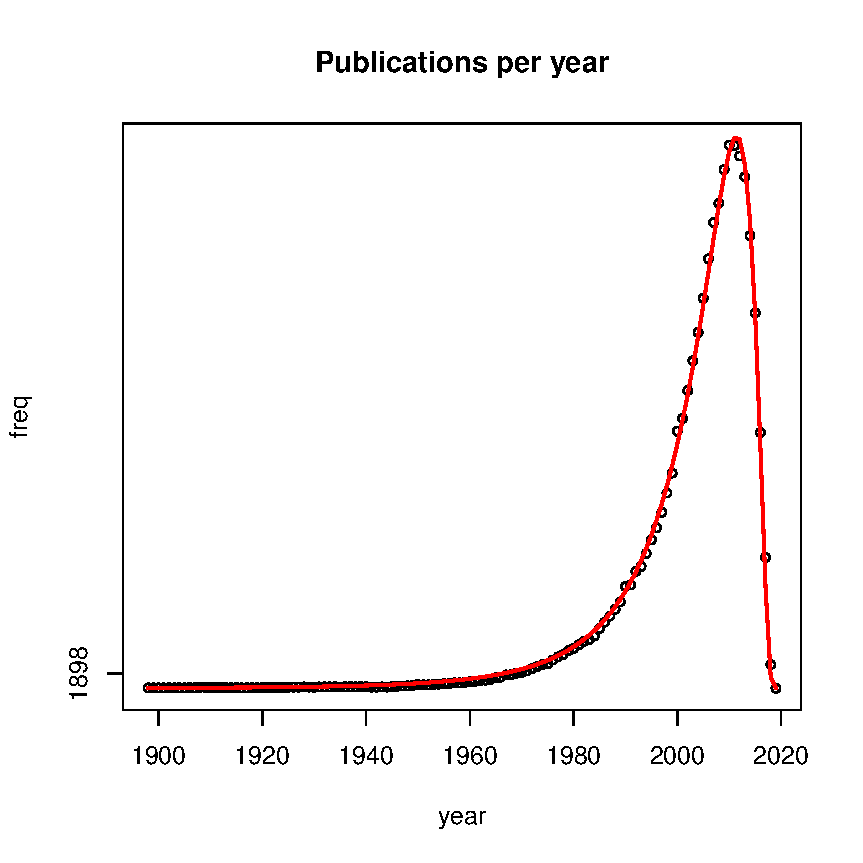
\includegraphics[width=75mm]{pubYear.pdf}
\end{center}
\end{frame}


\begin{frame}[fragile]
\frametitle{Cite network\label{maxin}\\ \normalsize Indegree distribution}

\begin{center}
%\includegraphics[width=43mm,viewport=100 40 405 550,clip=]{island2.pdf}
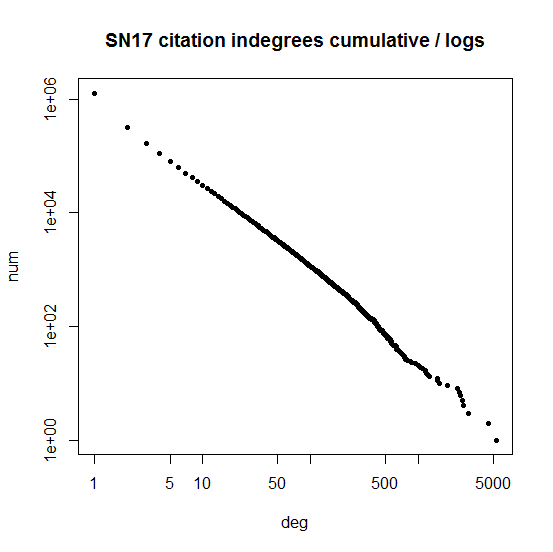
\includegraphics[width=50mm]{CiteIndegCum.png}
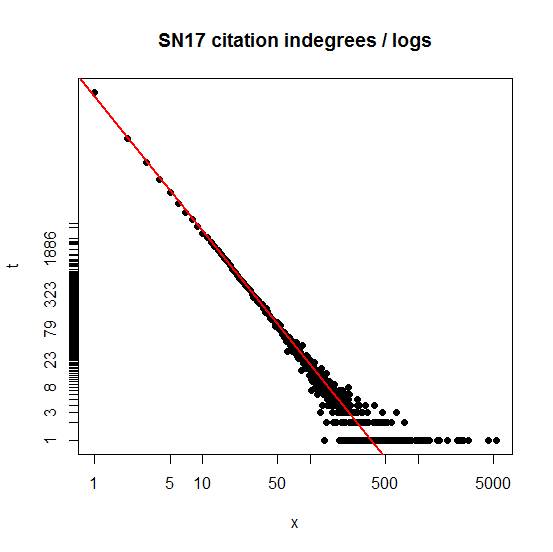
\includegraphics[width=50mm]{CiteIndegplfit.png}
\end{center}

\end{frame}


\begin{frame}[fragile]
\frametitle{Cite net\label{maxin}\\ \normalsize The most cited works - indegree}

\renewcommand{\arraystretch}{0.82}
\tiny
\begin{tabular}{r|r|l||r|r|l}
i	& freq	& id	                                           & i	& freq & id \\ \hline
1& 	5348& 	WASSERMA\_S(1994):& 	31& 	734& 	NEWMAN\_M(2001)98:404	\\
2& 	4471& 	GRANOVET\_M(1973)78:1360& 	32& 	719& 	NEWMAN\_M(2010):	\\
3& 	2906& 	WATTS\_D(1998)393:440& 	33& 	701& 	PORTES\_A(1998)24:1	\\
4& 	2614& 	BARABASI\_A(1999)286:509& 	34& 	687& 	BLEI\_D(2003)3:993	\\
5& 	2561& 	FREEMAN\_L(1979)1:215& 	35& 	670& 	BURT\_R(2004)110:349	\\
6& 	2447& 	BOYD\_D(2007)13:210& 	36& 	654& 	HANSEN\_M(1999)44:82	\\
7& 	2429& 	MCPHERSO\_M(2001)27:415& 	37& 	639& 	PALLA\_G(2005)435:814	\\
8& 	2330& 	BURT\_R(1992):& 	38& 	634& 	CLAUSET\_A(2004)70:066111	\\
9& 	1886& 	COLEMAN\_J(1988)94:95& 	39& 	629& 	BONACICH\_P(1987)92:1170	\\
10& 	1572& 	NEWMAN\_M(2003)45:167& 	40& 	628& 	ERDOS\_P(1959)6:290	\\
11& 	1520& 	GIRVAN\_M(2002)99:7821& 	41& 	628& 	UZZI\_B(1997)42:35	\\
12& 	1510& 	PUTNAM\_R(2000):& 	42& 	628& 	ROGERS\_E(2003):	\\
13& 	1285& 	ALBERT\_R(2002)74:47& 	43& 	613& 	PUTNAM\_R(1993):	\\
14& 	1240& 	GRANOVET\_M(1985)91:481& 	44& 	593& 	BERKMAN\_L(1979)109:186	\\
15& 	1192& 	SCOTT\_J(2000):& 	45& 	583& 	ZACHARY\_W(1977)33:452	\\
16& 	1171& 	EVERETT\_M(2002):& 	46& 	572& 	BORGATTI\_S(2009)323:892	\\
17& 	1166& 	NEWMAN\_M(2004)69:026113& 	47& 	569& 	NEWMAN\_M(2001)64:025102	\\
18& 	1093& 	COLEMAN\_J(1990):& 	48& 	565& 	BURT\_R(2005):	\\
19& 	1058& 	STEINFIE\_C(2007)12:1143& 	49& 	561& 	ADLER\_P(2002)27:17	\\
20& 	1034& 	FORTUNAT\_S(2010)486:75& 	50& 	559& 	CHRISTAK\_N(2008)358:2249	\\
21& 	999& 	BORGATTI\_S(2002):& 	51& 	555& 	ROGERS\_E(1995):	\\
22& 	945& 	CHRISTAK\_N(2007)357:370& 	52& 	554& 	MILGRAM\_S(1967)1:61	\\
23& 	867& 	FREEMAN\_L(1977)40:35& 	53& 	553& 	BARON\_R(1986)51:1173	\\
24& 	854& 	HANNEMAN\_R(2005):& 	54& 	550& 	GRANOVET\_M(1978)83:1420	\\
25& 	800& 	LIN\_N(2001):& 	55& 	539& 	FISCHER\_C(1982):	\\
26& 	757& 	KAPLAN\_A(2010)53:59& 	56& 	537& 	BRIN\_S(1998)30:107	\\
27& 	756& 	BLONDEL\_V(2008):P10008& 	57& 	524& 	MARSDEN\_P(1990)16:435	\\
28& 	742& 	NAHAPIET\_J(1998)23:242& 	58& 	523& 	KEMP\_D(2003):137	\\
29& 	740& 	FORNELL\_C(1981)18:39& 	59& 	523& 	KLEINBER\_J(1999)46:604	\\
30& 	740& 	NEWMAN\_M(2006)103:8577& 	60& 	517& 	BOCCALET\_S(2006)424:175	\\ \hline
\end{tabular}

\end{frame}

\begin{frame}[fragile]
\frametitle{Cite net \label{maxin}\\ \normalsize The most citing work - outdegree}
\small
\renewcommand{\arraystretch}{0.82}
\tiny
\begin{tabular}{r|r|l||r|r|l}
i&	freq& 	id&	i&	freq&	id	\\ \hline 
1& 	1572& 	CHAPMAN\_C(2016):1&	11& 	731& 	TSATSOU\_P(2014):1\\
2& 	1406& 	HRUSCHKA\_D(2010)5:1&	12& 	654& 	GOODALE\_E(2017):IX\\
3& 	1293& 	COWARD\_F(2015):1&	13& 	649& 	PEPPER\_G(2017)40:S0140525X1700190X\\
4& 	1254& 	FITZGERA\_P(2008):1&	14& 	632& 	STROM\_R(2012):1\\
5& 	1207& 	DAVIES\_N(2015):V&	15& 	613& 	SCHACHNE\_G(2015)23:49\\
6& 	1055& 	MARSH\_C(2009):1&	16& 	597& 	COSTA\_L(2011)60:329\\
7& 	942& 	YUS\_F(2011)213:1&	17& 	593& 	BRANDES\_U(2005)3418:1\\
8& 	929& 	BOCCALET\_S(2006)424:175&	18& 	586& 	ROBERTS\_J(2014):1\\
9& 	799& 	REEVES\_M(2017):1&	19& 	557& 	GUNTER\_B(2016):1\\
10& 	768& 	GROSS\_J(2007):1&	20& 	547& 	CASTELLA\_C(2009)81:591\\ \hline 
\end{tabular}

%\footnotesize
\begin{itemize}
\item MUIJS, D., Reynolds, D.,  CHAPMAN, C. (2015). Educational effectiveness and improvement research and practice: The emergence of the discipline. In The Routledge International Handbook of Educational Effectiveness and Improvement (pp. 33-56). Routledge.

\item  Hruschka, D. J. (2010). Friendship: Development, ecology, and evolution of a relationship (Vol. 5). Univ of California Press.

\item Coward, F., Hosfield, R., Pope, M.,  Wenban-Smith, F. (Eds.). (2015). Settlement, society and cognition in human evolution. Cambridge University Press.

\item Fitzgerald, P.,  Lambkin, B. (2008). Migration in Irish history 1607-2007. Springer.

\item Davies, N.B. Animal Social Networks Foreword. In: Krause, J., James, R., Franks, D. W., Croft, D. P. (Eds.). (2015). Animal social networks. Oxford University Press, USA.

\item Marsh, C. J. (2009). Key concepts for understanding curriculum. Routledge.
\end{itemize}

\end{frame}

\begin{frame}[fragile]
\frametitle{WA net \label{numpap}\\ \normalsize Authors with the largest number of papers - indegree}

\renewcommand{\arraystretch}{0.82}
\tiny
\begin{center}
\begin{tabular}{l|l|l||l|l|l}
Rank& 	Value& 	Id& 	Rank& 	Value& 	Id\\  \hline   
1& 	1169& 	WANG\_Y& 	21& 	552& 	KIM\_H\\ 
2& 	883& 	ZHANG\_Y& 	22& 	550& 	CHEN\_J\\ 
3& 	868& 	CHEN\_Y& 	23& 	536& 	LIU\_X\\ 
4& 	847& 	LI\_Y& 	24& 	533& 	WANG\_L\\ 
5& 	838& 	WANG\_X& 	25& 	509& 	LI\_H\\ 
6& 	819& 	ZHANG\_J& 	26& 	490& 	KIM\_Y\\ 
7& 	788& 	WANG\_J& 	27& 	485& 	ZHANG\_Z\\ 
8& 	786& 	LIU\_Y& 	28& 	474& 	WANG\_Z\\ 
9& 	766& 	LEE\_J& 	29& 	471& 	WANG\_S\\ 
10& 	765& 	LEE\_S& 	30& 	471& 	CHEN\_X\\ 
11& 	749& 	LI\_J& 	31& 	471& 	NEWMAN\_M\\ 
12& 	708& 	LI\_X& 	32& 	462& 	CHEN\_L\\ 
13& 	696& 	CHEN\_C& 	33& 	461& 	ZHANG\_L\\ 
14& 	690& 	KIM\_J& 	34& 	450& 	YANG\_Y\\ 
15& 	620& 	WANG\_H& 	35& 	450& 	ZHANG\_H\\ 
16& 	611& 	ZHANG\_X& 	36& 	432& 	WU\_J\\ 
17& 	611& 	LIU\_J& 	37& 	431& 	LEE\_H\\ 
18& 	570& 	CHEN\_H& 	38& 	420& 	LI\_Z\\ 
19& 	557& 	KIM\_S& 	39& 	420& 	WANG\_W\\ 
20& 	554& 	WANG\_C& 	40& 	417& 	LI\_L\\ \hline  
\end{tabular}
\end{center}

\medskip

The large number of Chinese authors in the list is a \href{https://en.wikipedia.org/wiki/List_of_common_Chinese_surnames}{"three Zhang, four Li"} effect. It is out of our resources to drill into this. We can only make a warning.

\end{frame}

\begin{frame}[fragile]
\frametitle{WA net \label{numpap}\\ \normalsize Number of authors in works - outdegree}
\renewcommand{\arraystretch}{0.82}
\tiny
\begin{center}
\begin{tabular}{l|l|l||l|l|l}
Cluster&  	Freq&  	Freq\% &  	Cluster&   Freq &	Freq\%\\ \hline   
1&  	1239496&  	95.5566&  	21&  	4&  	0.0003\\
2&  	18637&  	1.4368&  	22&  	3&  	0.0002\\
3&  	16661&  	1.2844&  	23&  	4&  	0.0003\\
4&  	10617&  	0.8185&  	24&  	2&  	0.0002\\
5&  	5759&  	0.4440&  	25&  	1&  	0.0001\\
6&  	2802&  	0.2160&  	26&  	2&  	0.0002\\
7&  	1322&  	0.1019&  	27&  	5&  	0.0004\\
8&  	686&  	0.0529&  	28&  	2&  	0.0002\\
9&  	384&  	0.0296&  	29&  	1&  	0.0001\\
10&  	247&  	0.0190&  	31&  	3&  	0.0002\\
11&  	155&  	0.0119&  	36&  	1&  	0.0001\\
12&  	90&  	0.0069&  	41&  	1&  	0.0001\\
13&  	70&  	0.0054&  	42&  	1&  	0.0001\\
14&  	54&  	0.0042&  	43&  	1&  	0.0001\\
15&  	32&  	0.0025&  	48&  	1&  	0.0001\\
16&  	12&  	0.0009&  	53&  	1&  	0.0001\\
17&  	14&  	0.0011&  	126&  	1&  	0.0001\\
18&  	9&  	0.0007&  	  & 	 & 	\\
19&  	6&  	0.0005&  	 &	 &	\\
20&  	2&  	0.0002&  	&	 &	\\ 
SUM &     &              &       &  1297133 & 100  \\ \hline   
\end{tabular}
\end{center}
\medskip

\footnotesize

Works with the largest number of authors:
\medskip
\begin{center}
\renewcommand{\arraystretch}{0.82}
\tiny 
\begin{tabular}{l|l|l|l|}
     Rank    & Freq & Id \\ \hline
         1   & 126  & WANG\_M(2016)34:828 \\
         2    & 53   & VASHISHT\_R(2012)7:0039808 \\ 
         3      & 48  & SNIJDERS\_T(2007)170:322 \\ 
         4     & 43  & GUSTAVSS\_A(2011)21:718  \\ 
         5    & 42   & DOLL\_L(1992)29:1 \\ 
         6   &41 &  MAGLIANO\_L(2006)15:219 \\ \hline
\end{tabular}
\end{center}

\end{frame}

\begin{frame}[fragile]
\frametitle{WA net  \label{numpap}\\ \normalsize Works with the largest number of authors - outdegree}

Sharing and community curation of mass spectrometry data with Global Natural Products Social Molecular Networking / Nature Biotechnology volume 34, pages 828–837 (2016)
\medskip

\renewcommand{\arraystretch}{0.82}
\tiny
Mingxun Wang, Jeremy J Carver, Vanessa V Phelan, Laura M Sanchez, Neha Garg, Yao Peng, Don Duy Nguyen, Jeramie Watrous, Clifford A Kapono, Tal Luzzatto-Knaan, Carla Porto, Amina Bouslimani, Alexey V Melnik, Michael J Meehan, Wei-Ting Liu, Max Crüsemann, Paul D Boudreau, Eduardo Esquenazi, Mario Sandoval-Calderón, Roland D Kersten, Laura A Pace, Robert A Quinn, Katherine R Duncan, Cheng-Chih Hsu, Dimitrios J Floros, Ronnie G Gavilan, Karin Kleigrewe, Trent Northen, Rachel J Dutton, Delphine Parrot, Erin E Carlson, Bertrand Aigle, Charlotte F Michelsen, Lars Jelsbak, Christian Sohlenkamp, Pavel Pevzner, Anna Edlund, Jeffrey McLean, Jörn Piel, Brian T Murphy, Lena Gerwick, Chih-Chuang Liaw, Yu-Liang Yang, Hans-Ulrich Humpf, Maria Maansson, Robert A Keyzers, Amy C Sims, Andrew R Johnson, Ashley M Sidebottom, Brian E Sedio, Andreas Klitgaard, Charles B Larson, Cristopher A Boya P, Daniel Torres-Mendoza, David J Gonzalez, Denise B Silva, Lucas M Marques, Daniel P Demarque, Egle Pociute, Ellis C O'Neill, Enora Briand, Eric J N Helfrich, Eve A Granatosky, Evgenia Glukhov, Florian Ryffel, Hailey Houson, Hosein Mohimani, Jenan J Kharbush, Yi Zeng, Julia A Vorholt, Kenji L Kurita, Pep Charusanti, Kerry L McPhail, Kristian Fog Nielsen, Lisa Vuong, Maryam Elfeki, Matthew F Traxler, Niclas Engene, Nobuhiro Koyama, Oliver B Vining, Ralph Baric, Ricardo R Silva, Samantha J Mascuch, Sophie Tomasi, Stefan Jenkins, Venkat Macherla, Thomas Hoffman, Vinayak Agarwal, Philip G Williams, Jingqui Dai, Ram Neupane, Joshua Gurr, Andrés M C Rodríguez, Anne Lamsa, Chen Zhang, Kathleen Dorrestein, Brendan M Duggan, Jehad Almaliti, Pierre-Marie Allard, Prasad Phapale, Louis-Felix Nothias, Theodore Alexandrov, Marc Litaudon, Jean-Luc Wolfender, Jennifer E Kyle, Thomas O Metz, Tyler Peryea, Dac-Trung Nguyen, Danielle VanLeer, Paul Shinn, Ajit Jadhav, Rolf Müller, Katrina M Waters, Wenyuan Shi, Xueting Liu, Lixin Zhang, Rob Knight, Paul R Jensen, Bernhard Ø Palsson, Kit Pogliano, Roger G Linington, Marcelino Gutiérrez, Norberto P Lopes, William H Gerwick, Bradley S Moore, Pieter C Dorrestein, Nuno Bandeira.

\end{frame}




\begin{frame}[fragile]
\frametitle{WJ net \\ \normalsize The most used journals - indegree}

\renewcommand{\arraystretch}{0.82}
\tiny
\begin{tabular}{r|r|l||r|r|l}
Rank&   	Value&   	Id&   	Rank&   	Value&   	Id \\ \hline
1&   	7080&   	LECT NOTES COMPUT SC&   	31&   	1258&   	AM J PSYCHIAT\\   
2&   	3859&   	SOC SCI MED&   	32&   	1221&   	J BUS RES\\   
3&   	3408&   	J PERS SOC PSYCHOL&   	33&   	1217&   	MANAGE SCI\\   
4&   	2719&   	COMPUT HUM BEHAV&   	34&   	1185&   	ACAD MANAGE REV\\   
5&   	2631&   	SCIENCE&   	35&   	1182&   	J CONSULT CLIN PSYCH\\   
6&   	2602&   	AM J PUBLIC HEALTH&   	36&   	1151&   	ORGAN SCI\\   
7&   	2599&   	P NATL ACAD SCI USA&   	37&   	1150&   	ADDICTION\\   
8&   	2208&   	NATURE&   	38&   	1143&   	STRATEGIC MANAGE J\\   
9&   	2058&   	AM SOCIOL REV&   	39&   	1087&   	J GERONTOL B-PSYCHOL\\   
10&   	1945&   	PHYSICA A&   	40&   	1075&   	PEDIATRICS\\   
11&   	1815&   	ANIM BEHAV&   	41&   	1055&   	AM J EPIDEMIOL\\   
12&   	1778&   	JAMA-J AM MED ASSOC&   	42&   	1050&   	COMPUT EDUC\\   
13&   	1763&   	LANCET&   	43&   	1022&   	DEV PSYCHOL\\   
14&   	1759&   	SCIENTOMETRICS&   	44&   	1022&   	PSYCHOL BULL\\   
15&   	1734&   	AM J SOCIOL&   	45&   	1007&   	J ADOLESCENT HEALTH\\   
16&   	1703&   	ACAD MANAGE J&   	46&   	997&   	J MARKETING\\   
17&   	1632&   	LECT NOTES ARTIF INT&   	47&   	996&   	ARCH GEN PSYCHIAT\\   
18&   	1573&   	J APPL PSYCHOL&   	48&   	994&   	AIDS BEHAV\\   
19&   	1551&   	SOC NETWORKS&   	49&   	972&   	PERS INDIV DIFFER\\   
20&   	1509&   	AM ECON REV&   	50&   	949&   	PERS SOC PSYCHOL B\\   
21&   	1433&   	J MARRIAGE FAM&   	51&   	947&   	J BUS ETHICS\\   
22&   	1400&   	BRIT MED J&   	52&   	939&   	J MARKETING RES\\   
23&   	1399&   	CHILD DEV&   	53&   	925&   	INFORM SCIENCES\\   
24&   	1373&   	EXPERT SYST APPL&   	54&   	916&   	HARVARD BUS REV\\   
25&   	1365&   	NEW ENGL J MED&   	55&   	915&   	IEEE T KNOWL DATA EN\\   
26&   	1363&   	COMMUN ACM&   	56&   	901&   	DRUG ALCOHOL DEPEN\\   
27&   	1355&   	RES POLICY&   	57&   	900&   	WORLD DEV\\   
28&   	1279&   	GERONTOLOGIST&   	58&   	899&   	AM J PREV MED\\   
29&   	1275&   	BRIT J PSYCHIAT&   	59&   	895&   	ADDICT BEHAV\\   
30&   	1271&   	SOC FORCES&   	60&   	893&   	J CONSUM RES\\  \hline
\end{tabular}

\end{frame}


\begin{frame}[fragile]
\frametitle{WK net \\ \normalsize The most used keywords - indegree}


\renewcommand{\arraystretch}{0.82}
\tiny
\begin{center}
\begin{tabular}{r|r|l||r|r|l}
Rank&  	Value&  	Id&  	Rank&  	Value&  	Id\\ \hline
1&  	51333&  	social&  	31&  	3485&  	structure\\
2&  	46191&  	network&  	32&  	3479&  	life\\
3&  	11751&  	analysis&  	33&  	3444&  	risk\\
4&  	10219&  	model&  	34&  	3358&  	research\\
5&  	8104&  	community&  	35&  	3143&  	learn\\
6&  	8090&  	use&  	36&  	3116&  	influence\\
7&  	7596&  	base&  	37&  	3054&  	student\\
8&  	7439&  	information&  	38&  	3054&  	impact\\
9&  	7061&  	health&  	39&  	3049&  	perspective\\
10&  	7023&  	behavior&  	40&  	3042&  	complex\\
11&  	6745&  	online&  	41&  	3024&  	theory\\
12&  	6087&  	networking&  	42&  	2859&  	organization\\
13&  	5833&  	media&  	43&  	2828&  	relationship\\
14&  	5404&  	support&  	44&  	2802&  	algorithm\\
15&  	5101&  	communication&  	45&  	2776&  	education\\
16&  	5013&  	study&  	46&  	2714&  	group\\
17&  	4759&  	datum&  	47&  	2704&  	mobile\\
18&  	4376&  	management&  	48&  	2698&  	tie\\
19&  	4372&  	internet&  	49&  	2695&  	adult\\
20&  	4164&  	knowledge&  	50&  	2633&  	approach\\
21&  	4126&  	user&  	51&  	2608&  	care\\
22&  	4023&  	facebook&  	52&  	2551&  	adolescent\\
23&  	3984&  	technology&  	53&  	2479&  	role\\
24&  	3907&  	site&  	54&  	2472&  	state\\
25&  	3888&  	web&  	55&  	2467&  	innovation\\
26&  	3855&  	self&  	56&  	2434&  	pattern\\
27&  	3784&  	graph&  	57&  	2385&  	effect\\
28&  	3676&  	performance&  	58&  	2339&  	people\\
29&  	3534&  	service&  	59&  	2333&  	trust\\
30&  	3512&  	dynamics&  	60&  	2332&  	family\\ \hline
\end{tabular}
\end{center}

\end{frame}

\section{Citation network}  

%******************************************************************************

\begin{frame}[fragile]
\frametitle{Cite net \\ \normalsize Boundary problem}
\small 

The network Cite has 1297133  nodes and 2753767 arcs.
\medskip

\begin{tabular}{r|r|r|r|r|}
 Cluster &       Freq &    Freq\%  &  CumFreq &  CumFreq\% \\ \hline
 0     & 41954   &  3.2344     & 41954   &  3.2344  \\ 
1   &  933315  &  71.9521   &  975269  & 75.1865  \\
2   &  154895   & 11.9413   & 1130164  &  87.1278 \\
3   &  58141    & 4.4823   & 1188305   & 91.6101  \\ 
4   &  29885   & 2.3039  & 1218190  & 93.9140 \\  
5   &  17651   & 1.3608   & 1235841  & 95.2748  \\ \hline
\end{tabular}

\medskip

Most of nodes are terminal $(DCr=0)$ or nodes cited only once (indegree=1). We decided (boundary problem) to include in our networks nodes with $DCr > 0$ or $\indeg > 2$ (partition boundary). They determine a subnetwork CiteB with  222 086 nodes and 1 521 434 arcs.

\end{frame}

\begin{frame}[fragile]
\frametitle{Cite net \\ \normalsize Components}
\small 
To get an acyclic network we applied the \keyw{preprint transformation} to CiteB. The resulting network CiteT has 222 189 nodes and 1 521 658 arcs. 

We computed the SPC weights on network arcs, and determined 
\begin{itemize}
\item CPM path (Main path) = 59 nodes
\item Key-routes = 127 nodes  
\item SPC link islands [Line weights] of sizes [20, 200] = 5 islands of 138, 65, 13, 12, and 11 nodes  
\item SPC node islands [Vertex weights] of sizs  [20, 200] = 1 island of 200 nodes
\end{itemize}

\medskip 

We computed the Probabilistic flow on weighted network, and determined node islands [Vertex weights] of sizs  [10, 200] = 200 nodes

\end{frame}

\begin{frame}[fragile]
\frametitle{Strong components \\ \normalsize from SPC network}

\begin{center}
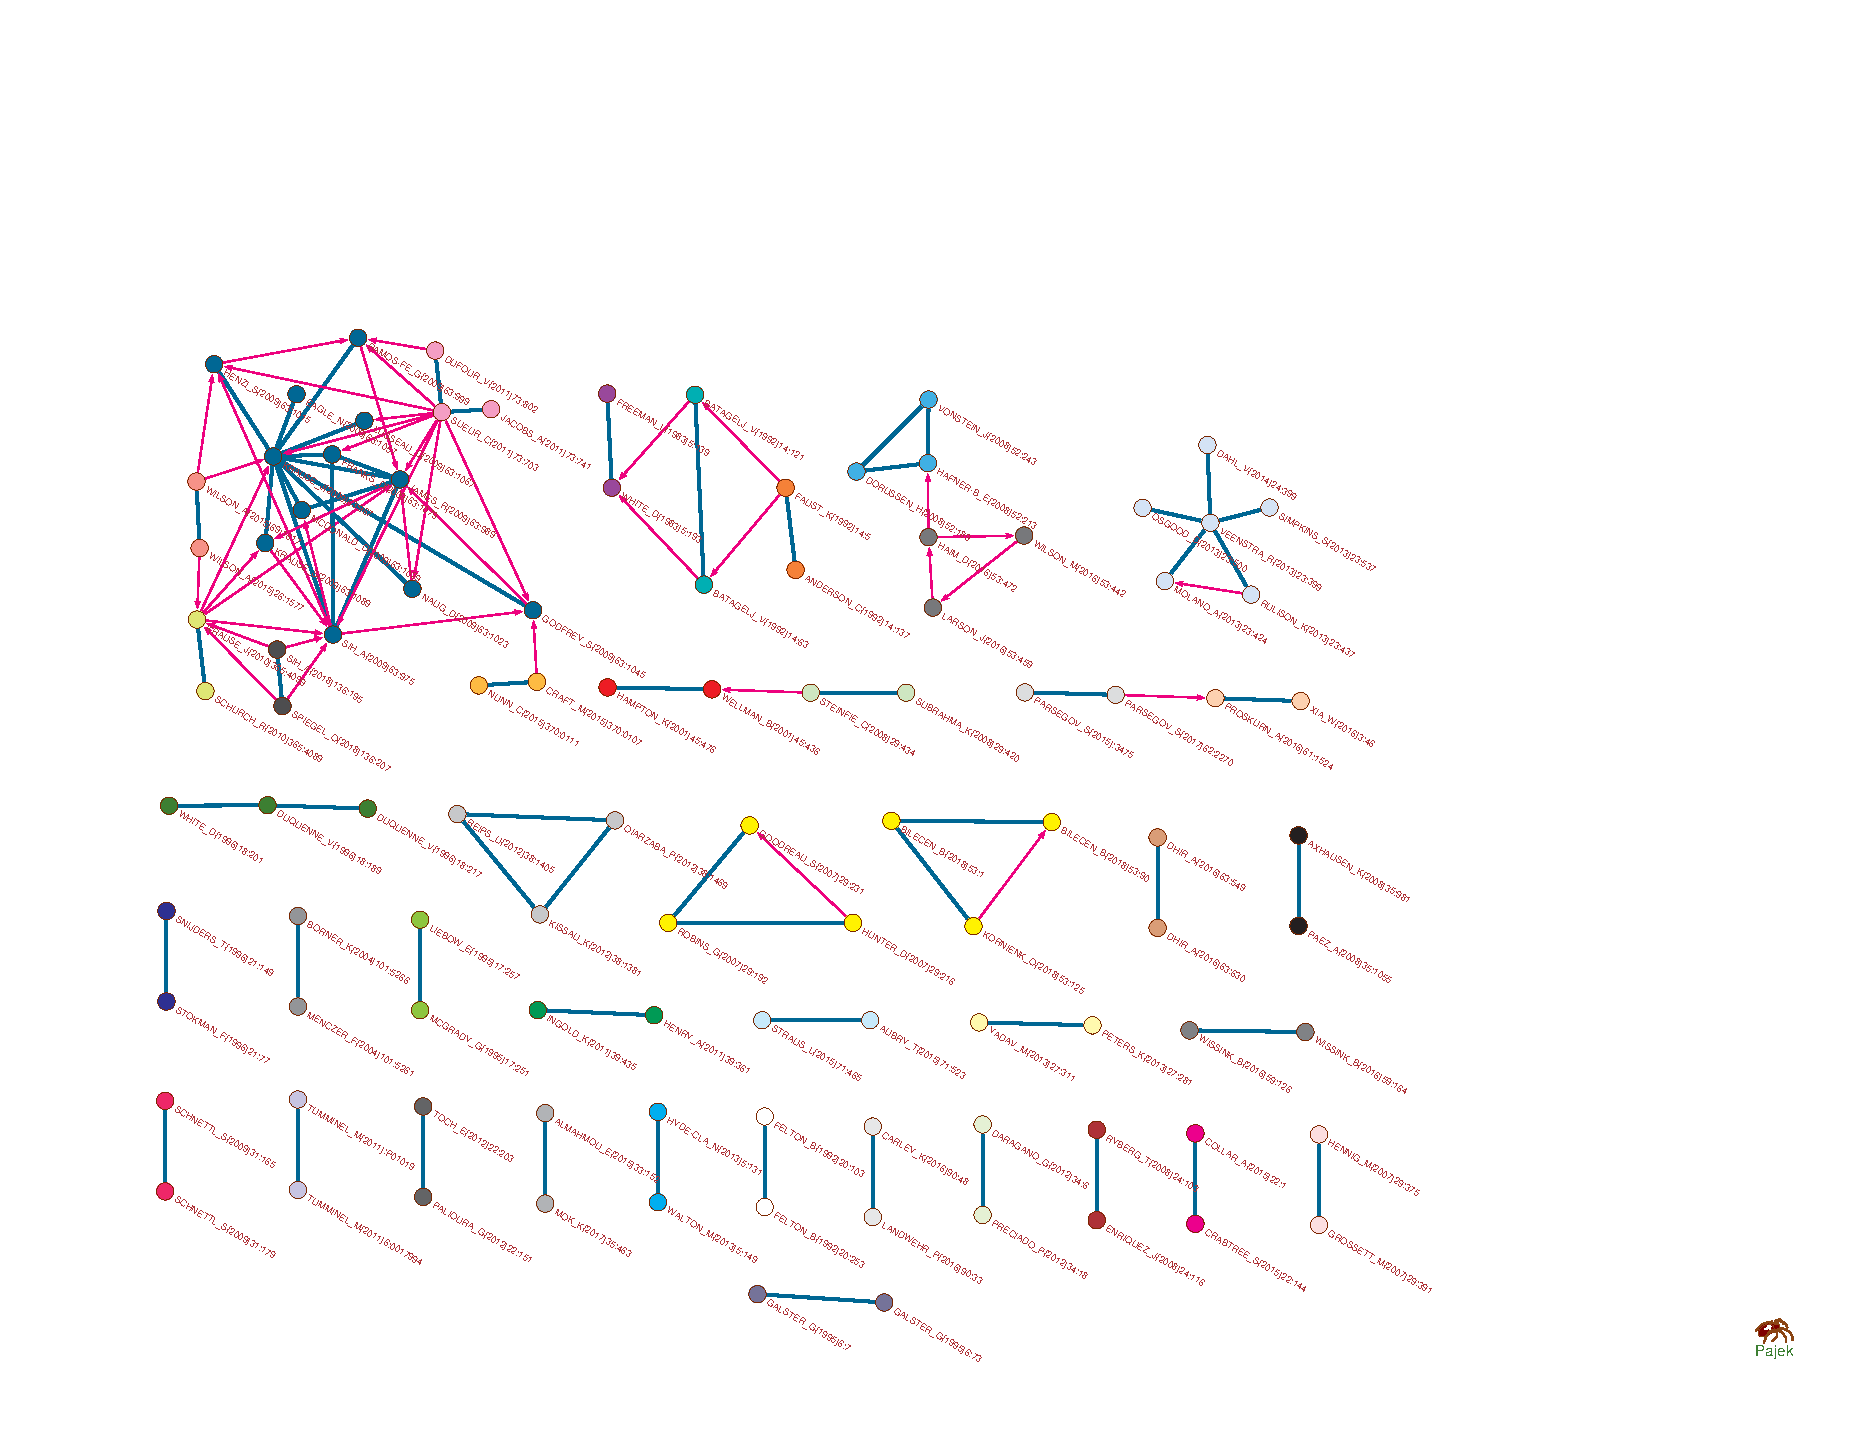
\includegraphics[width=80mm,viewport=90 34 690 535,clip=]{strong.pdf}
%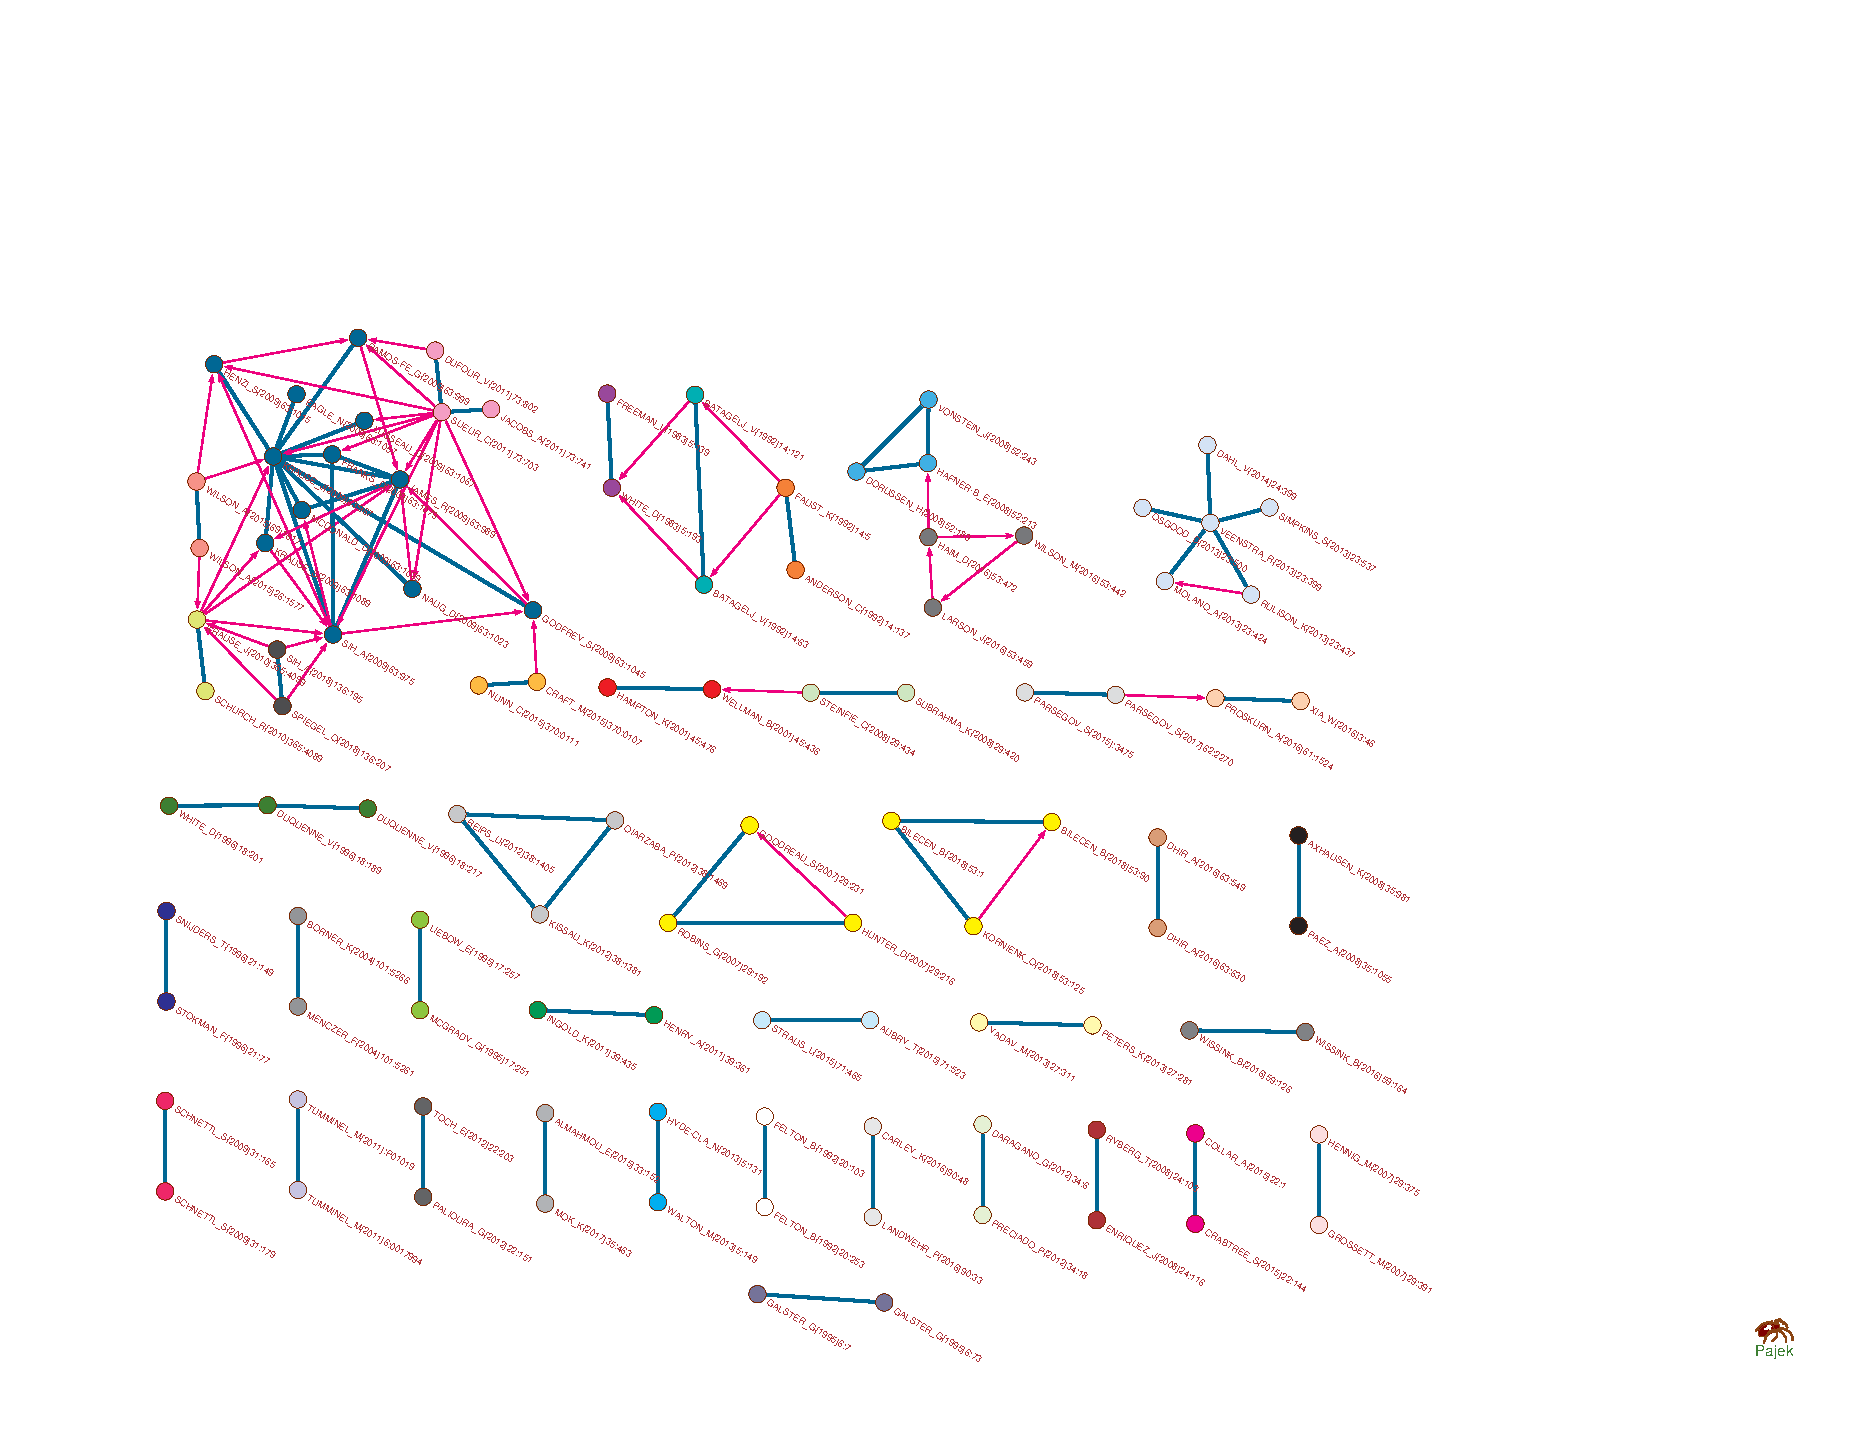
\includegraphics[width=100mm,viewport=90 320 670 535,clip=]{strong.pdf}
\end{center}

\end{frame}

\begin{frame}[fragile]
\frametitle{Main path, Key Routes, and Island 4 \\ \normalsize from SPC network}
\begin{center}

\includegraphics[width=9mm,viewport=120 27 235 682 ,clip=]{CPMpath.pdf}
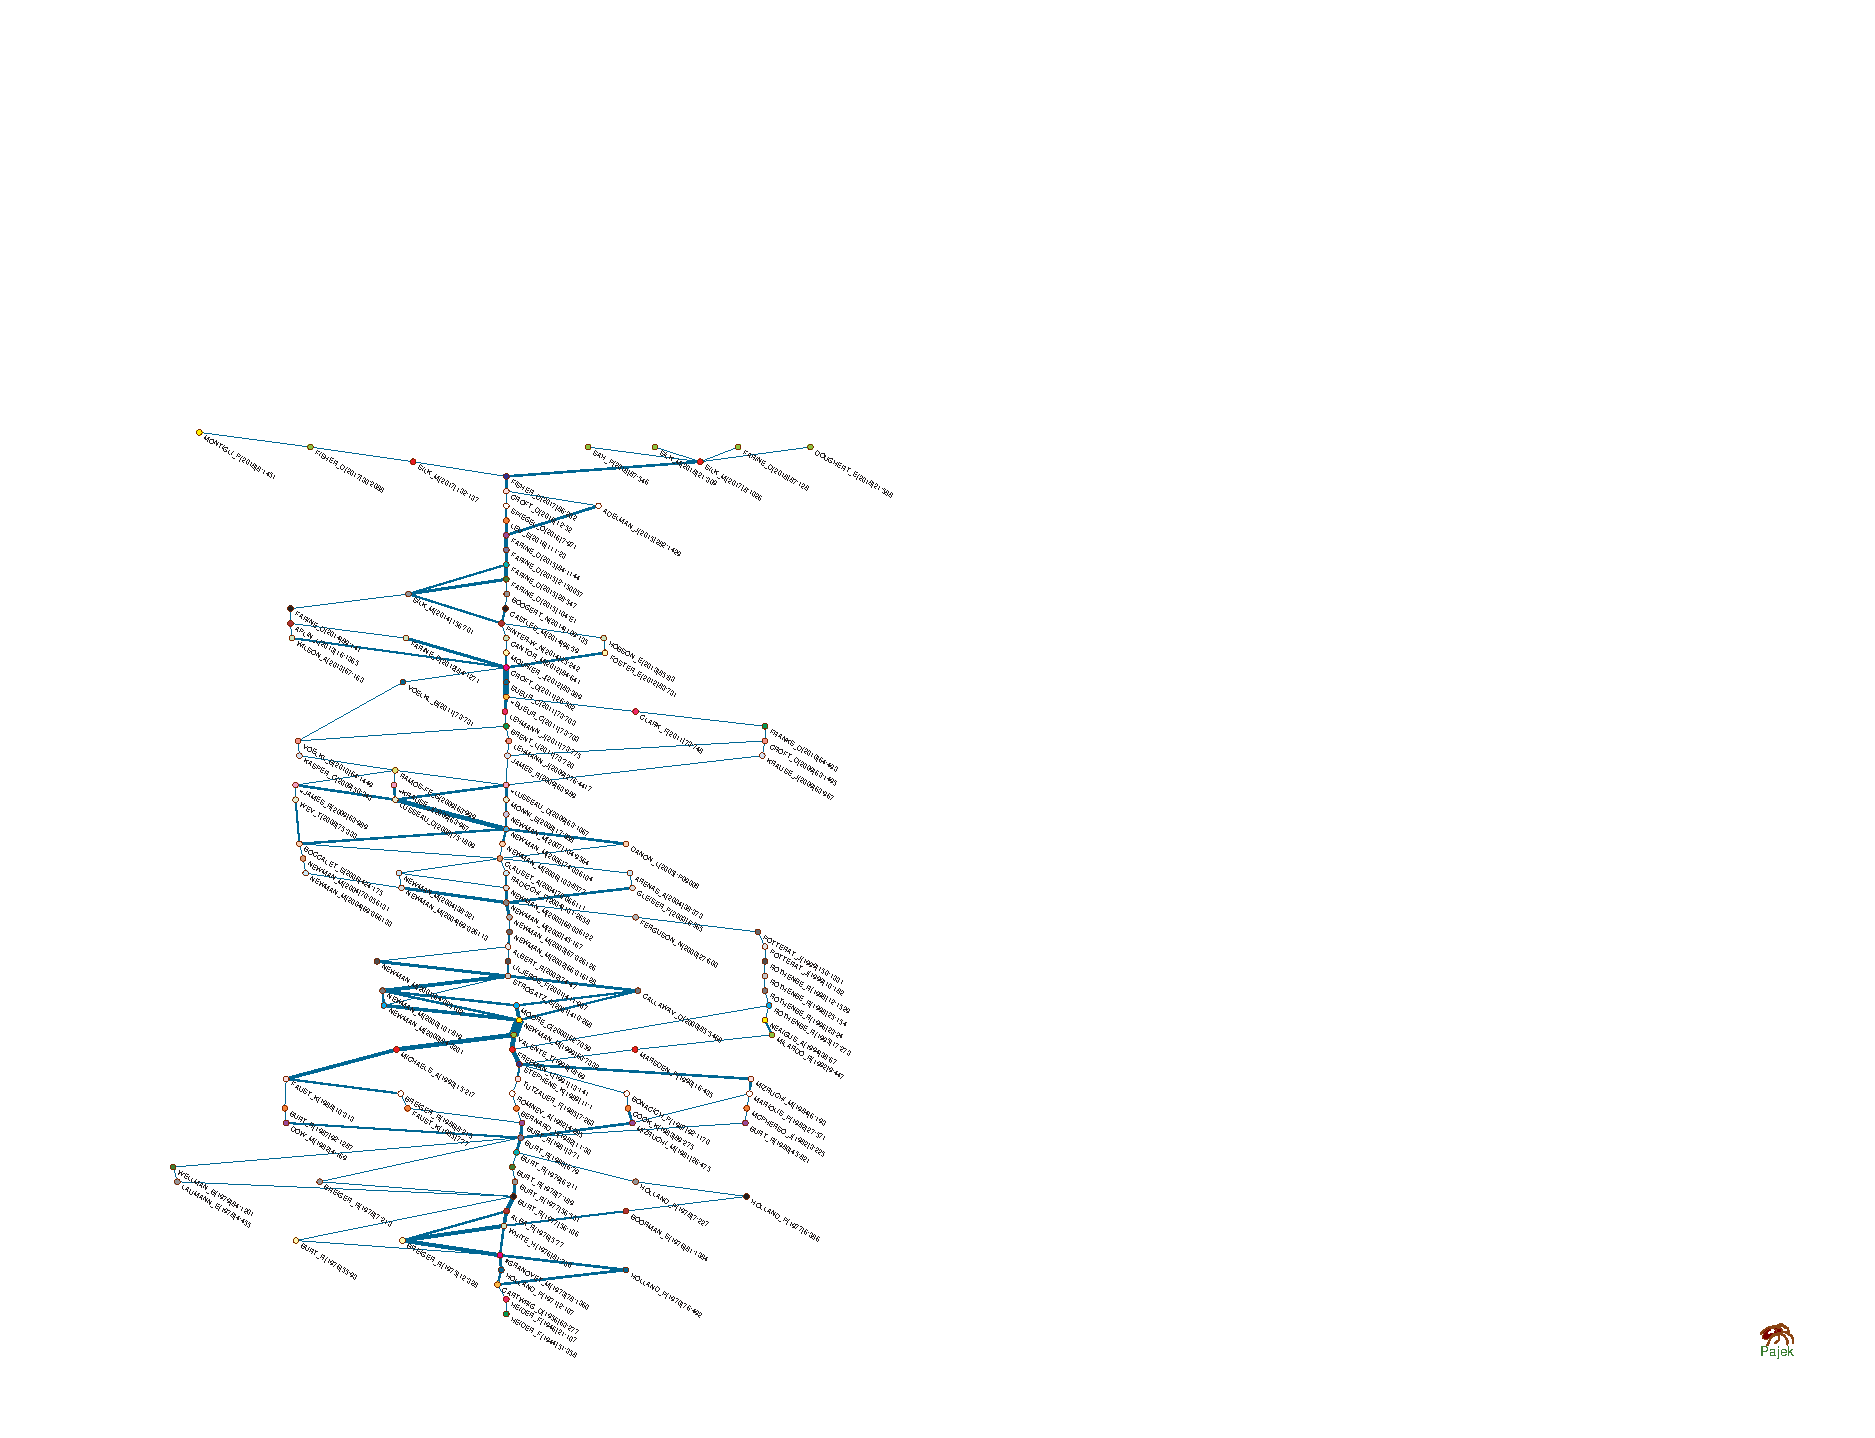
\includegraphics[width=40mm,viewport=75 37 440 590,clip=]{KeyRouteW.pdf}
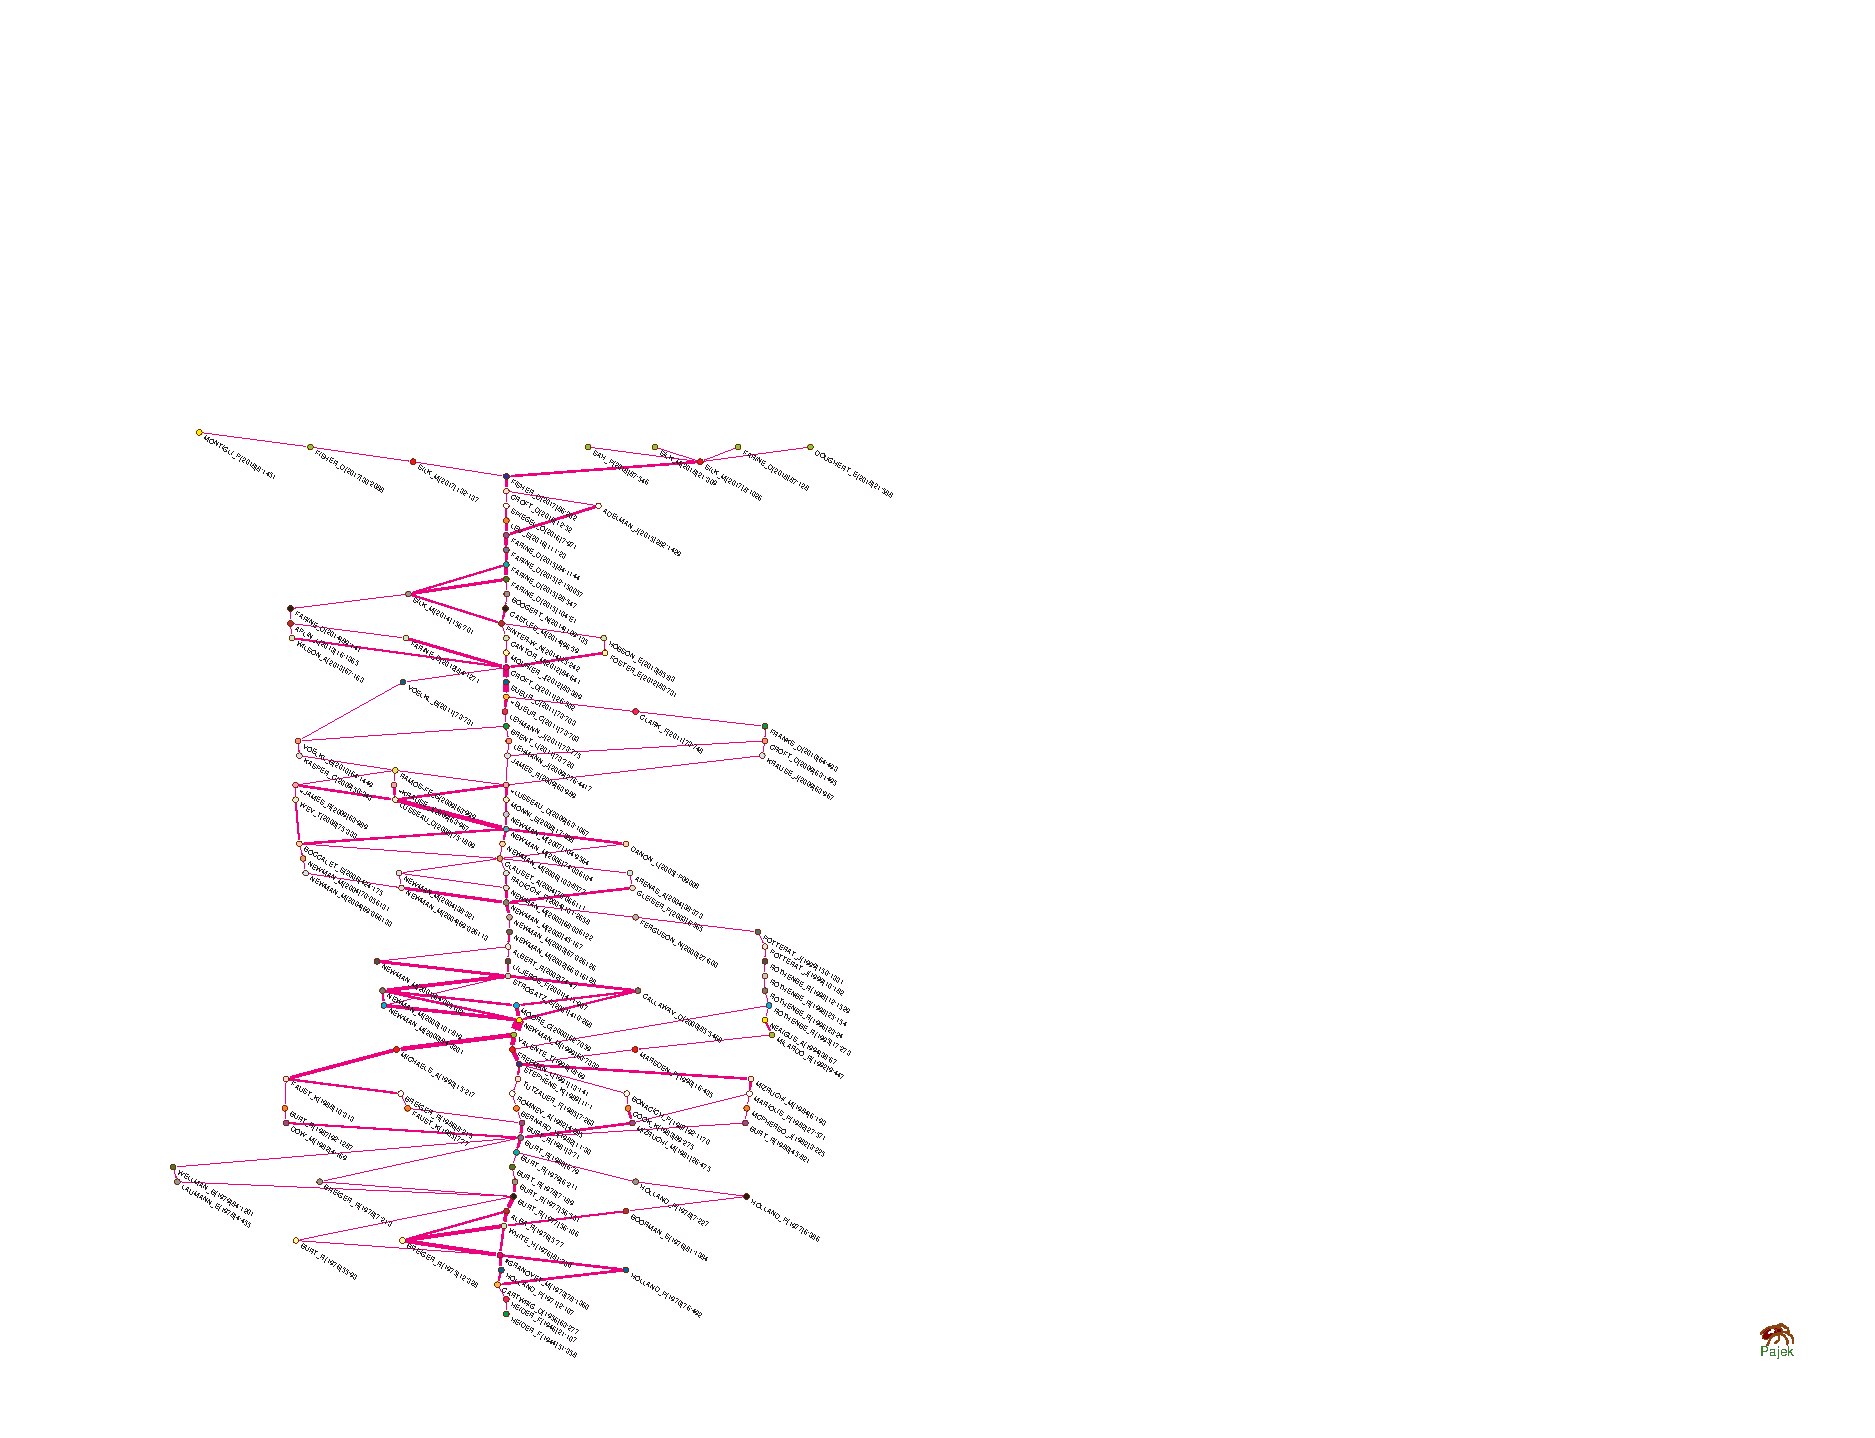
\includegraphics[width=37mm,viewport=75 40 400 600,clip=]{Island4w.pdf}
\end{center}

\end{frame}

\begin{frame}[fragile]
\frametitle{Islands 1-3, 4 \\ \normalsize from SPC network}
\begin{center}
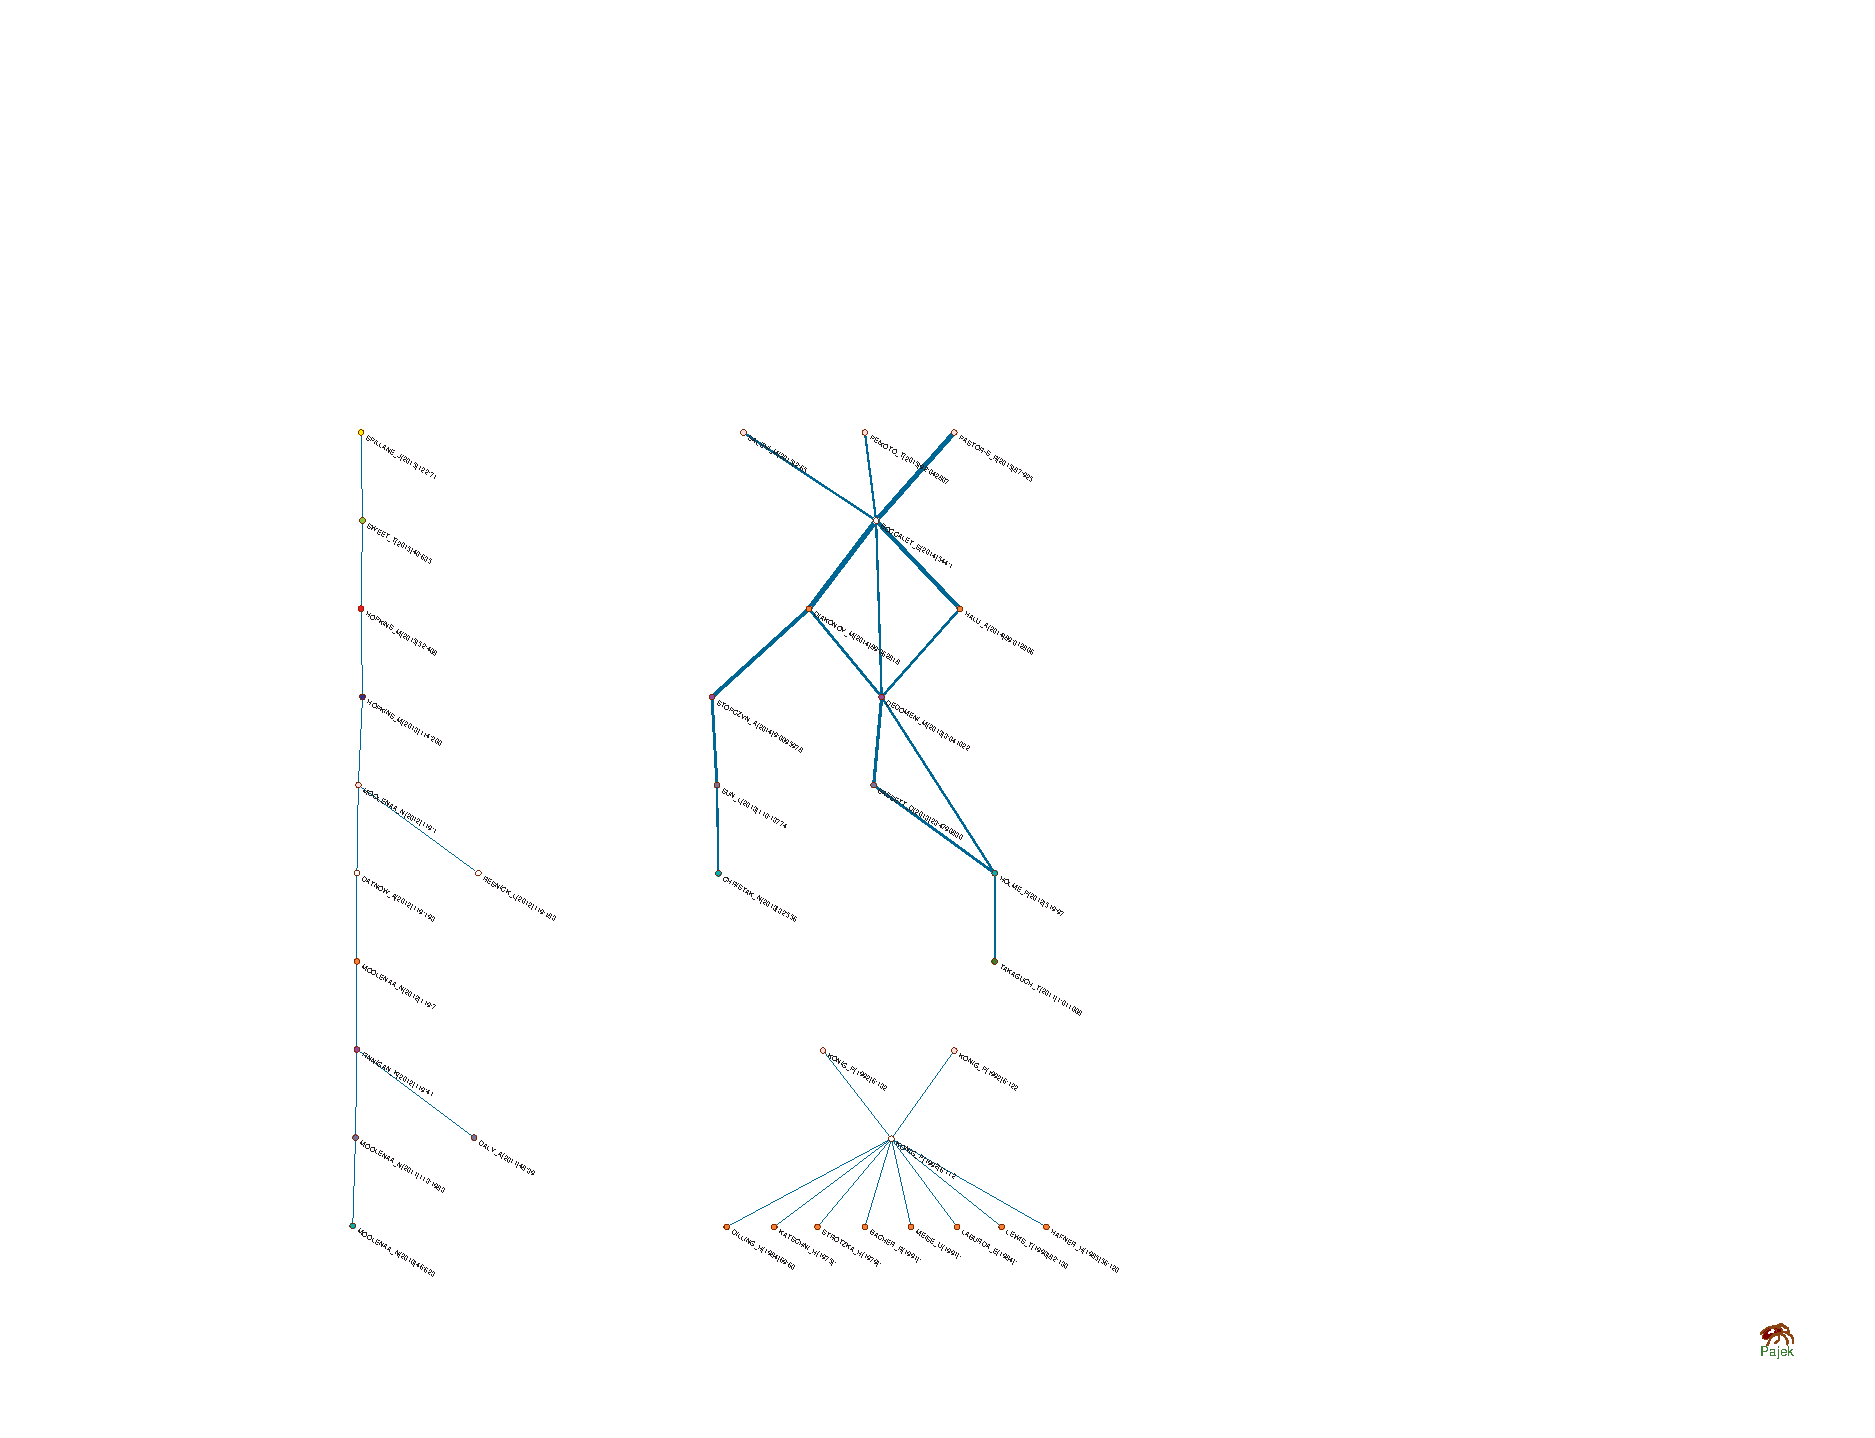
\includegraphics[width=40mm,viewport=160 75 540 488 ,clip=]{Island1-3w.pdf}
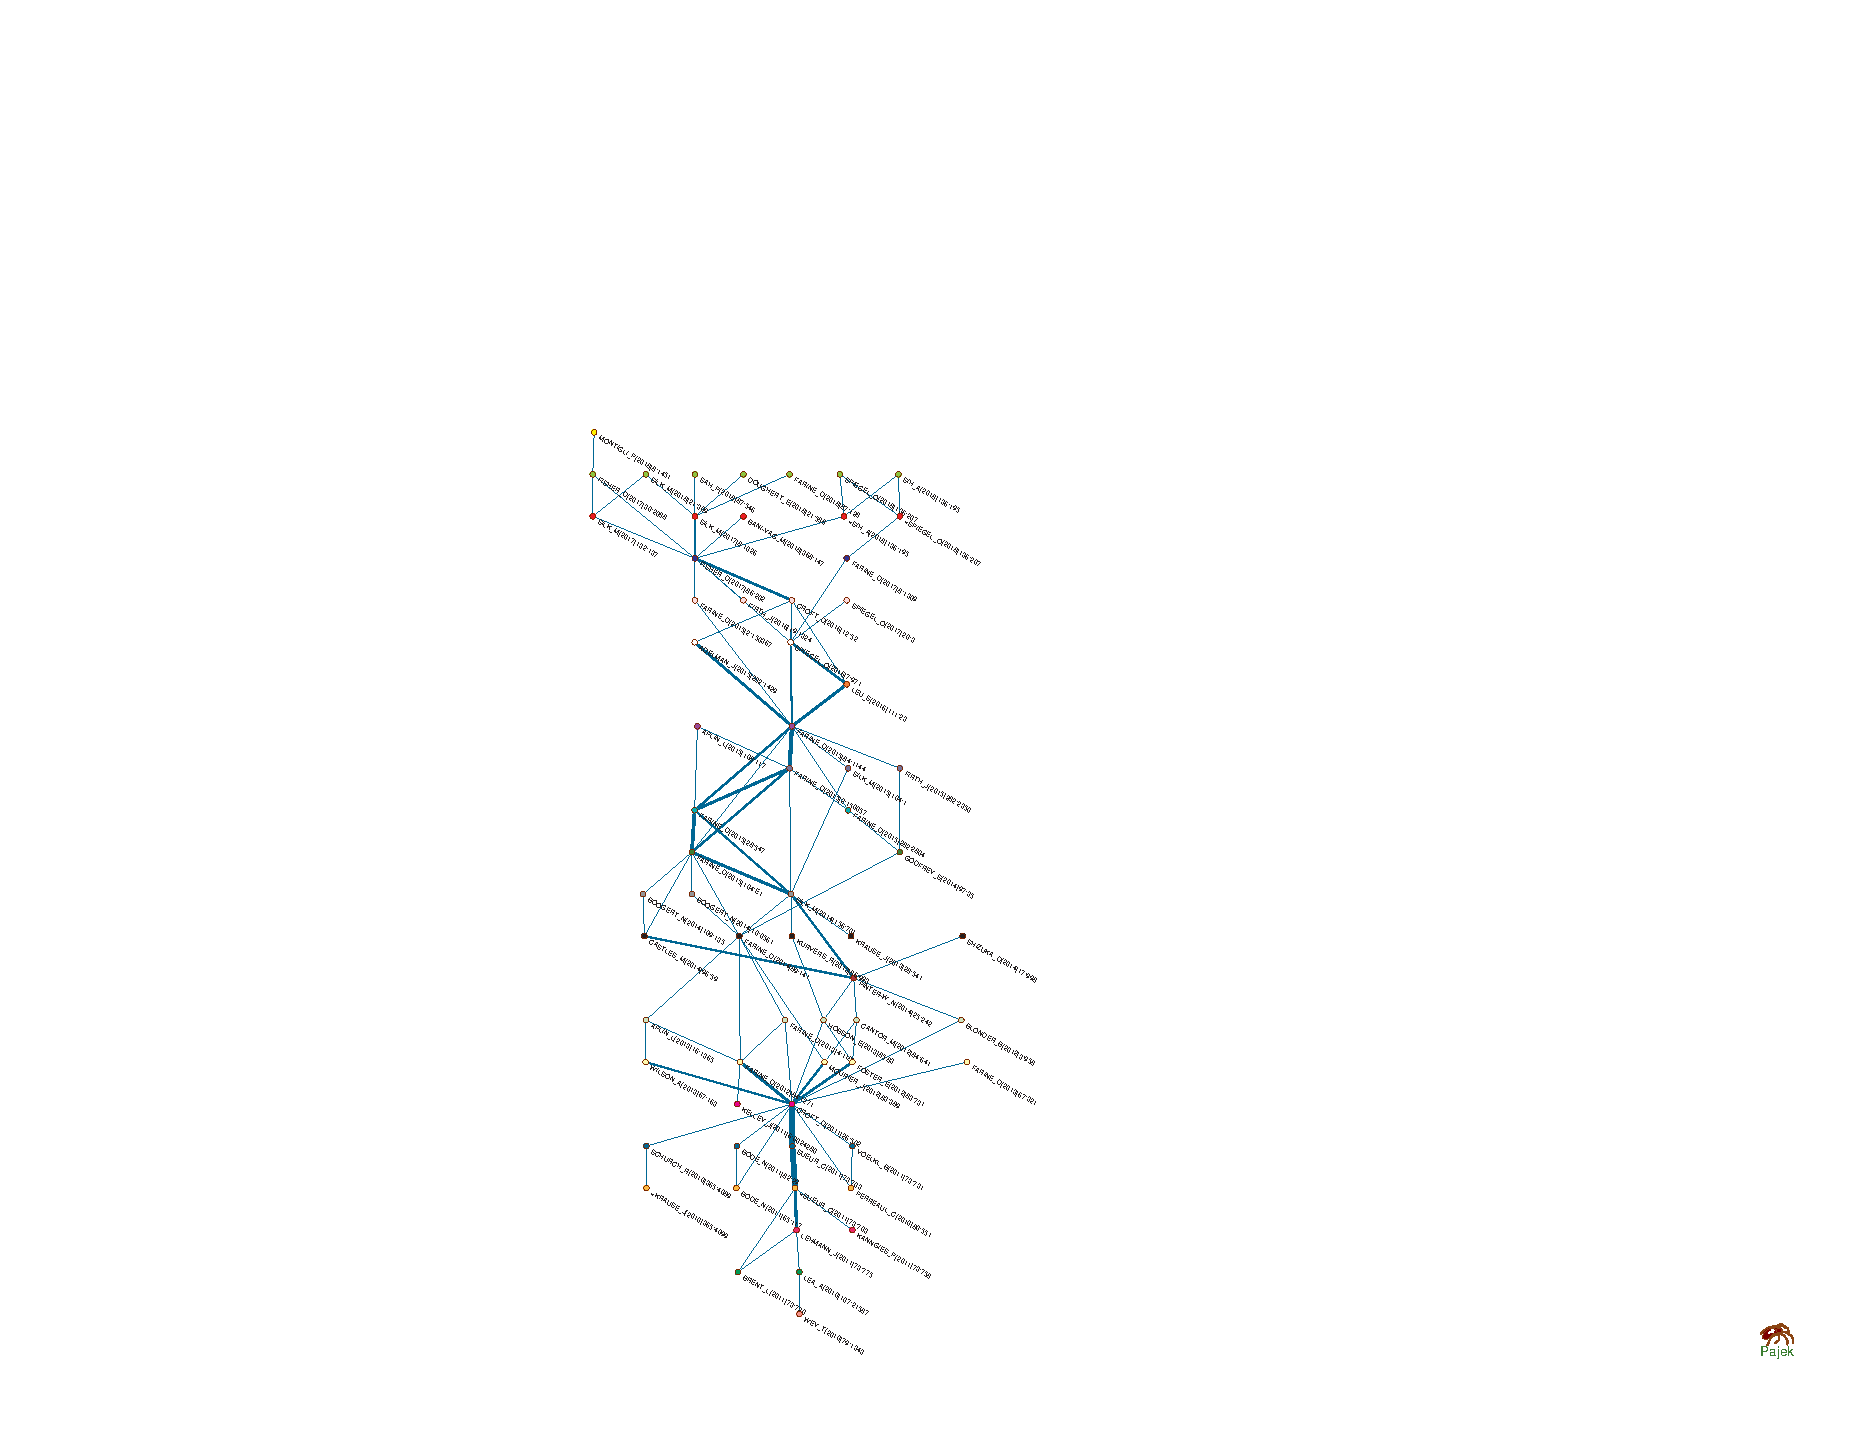
\includegraphics[width=40mm,viewport=280 37 500 488,clip=]{Island5w.pdf}
\end{center}

\end{frame}


\begin{frame}[fragile]
\frametitle{Most important works \\ \normalsize from Probabilistic  Flow network}
\small

\renewcommand{\arraystretch}{0.82}
\tiny
\begin{tabular}{c|c|l||c|c|l|l}
Rank&   	Value&   	Id&   	Rank&   	Value&   	Id\\ \hline
1&   	4691.7033&   	WASSERMA\_S(1994):&   	31&   	545.5328&   	BLONDEL\_V(2008):P10008\\
2&   	2941.1761&   	WATTS\_D(1998)393:440&   	32&   	527.9645&   	KATZ\_L(1953)18:39\\
3&   	2676.7765&   	GRANOVET\_M(1973)78:1360&   	33&   	526.3830&   	NEWMAN\_M(2010):\\
4&   	2445.6729&   	BOYD\_D(2007)13:210&   	34&   	520.1086&   	STROGATZ\_S(2001)410:268\\
5&   	2241.3353&   	BARABASI\_A(1999)286:509&   	35&   	517.8303&   	PALLA\_G(2005)435:814\\
6&   	1926.1505&   	FREEMAN\_L(1979)1:215&   	36&   	499.7478&   	CLAUSET\_A(2004)70:066111\\
7&   	1396.7653&   	GIRVAN\_M(2002)99:7821&   	37&   	497.4825&   	ERDOS\_P(1960)5:17\\
8&   	1299.3284&   	NEWMAN\_M(2003)45:167&   	38&   	488.1258&   	ROGERS\_E(2003):\\
9&   	1227.6464&   	MCPHERSO\_M(2001)27:415&   	39&   	485.0419&   	NEWMAN\_M(2006)103:8577\\
10&   	1158.1156&   	ALBERT\_R(2002)74:47&   	40&   	481.1530&   	COLEMAN\_J(1990):\\
11&   	1105.4924&   	SCOTT\_J(2000):&   	41&   	478.3532&   	BRIN\_S(1998)30:107\\
12&   	1098.3635&   	BURT\_R(1992):&   	42&   	477.1407&   	AMARAL\_L(2000)97:11149\\
13&   	1045.2931&   	MILGRAM\_S(1967)1:61&   	43&   	475.3617&   	ERDOS\_P(1959)6:290\\
14&   	1013.5490&   	NEWMAN\_M(2004)69:026113&   	44&   	465.2929&   	WATTS\_D(1999):\\
15&   	928.3289&   	KAPLAN\_A(2010)53:59&   	45&   	462.8299&   	LAVE\_J(1991):\\
16&   	878.0197&   	FREEMAN\_L(1977)40:35&   	46&   	460.1905&   	KLEINBER\_J(1999)46:604\\
17&   	852.0768&   	PUTNAM\_R(2000):&   	47&   	449.5945&   	SCOTT\_J(1991):\\
18&   	847.1235&   	COLEMAN\_J(1988)94:95&   	48&   	446.7720&   	BOLLOBAS\_B(1985):\\
19&   	835.6368&   	BLEI\_D(2003)3:993&   	49&   	442.9941&   	PAGE\_L(1999):\\
20&   	742.6433&   	GRANOVET\_M(1985)91:481&   	50&   	440.0067&   	NEWMAN\_M(2001)64:025102\\
21&   	731.1789&   	CHRISTAK\_N(2007)357:370&   	51&   	436.9754&   	NEWMAN\_M(2004)69:066133\\
22&   	727.1355&   	EVERETT\_M(2002):&   	52&   	431.0422&   	REDNER\_S(1998)4:131\\
23&   	726.4118&   	NEWMAN\_M(2001)98:404&   	53&   	429.5661&   	CHRISTAK\_N(2008)358:2249\\
24&   	719.2622&   	ALBERT\_R(1999)401:130&   	54&   	424.2269&   	ADOMAVIC\_G(2005)17:734\\
25&   	701.0592&   	O'REILLY\_T(2005):&   	55&   	424.0579&   	KEMP\_D(2003):137\\
26&   	669.0536&   	BORGATTI\_S(2002):&   	56&   	423.4092&   	DOMINGOS\_P(2001):57\\
27&   	667.5963&   	FORTUNAT\_S(2010)486:75&   	57&   	423.0635&   	MITCHELL\_J(1969):\\
28&   	633.3008&   	HANNEMAN\_R(2005):&   	58&   	415.6691&   	ALBERT\_R(2000)406:378\\
29&   	569.2848&   	STEINFIE\_C(2007)12:1143&   	59&   	415.3695&   	GLASER\_B(1967):\\
30&   	549.4440&   	ZACHARY\_W(1977)33:452&   	60&   	410.1489&   	ROGERS\_E(1995):\\ \hline
\end{tabular}

\end{frame}


\begin{frame}[fragile]
\frametitle{Main island\\ \normalsize from Probabilistic  Flow network}
\small

Prob flow pic 
%to be done 

\end{frame}

\begin{frame}[fragile]
\frametitle{Cite net\\ \normalsize Overlapping of components}
\small

\renewcommand{\arraystretch}{0.2}
\tiny
\begin{tabular}{c|l|l|l|l|}
i&   	name & title & jour & comp \\ \hline 
1&   	Granovet M &   	 Strength of weak ties&   	amer j sociol&   	1, 2, 4, 5, 6\\
2&   	Newman M&   	 The structure and function of complex networks&   	siam rev&   	1, 2, 4, 5, 6\\
3&   	Albert R&   	 Statistical mechanics of complex networks&   	rev mod phys&   	1, 2, 4, 5, 6\\
4&   	Boccaletti S&   	 Complex networks: structure and dynamics&   	phys rept&   	1, 2, 4, 5, 6\\
5&   	White H&   	 Soc. str. from mult. nets. Blockmodels &   	amer j sociol&   	1, 2, 4, 5, 6\\
6&   	Newman M&   	 Clustering and pref.l attach. in growing nets&   	phys rev e&   	1, 2, 4, 5, 6\\
7&   	Newman M&   	 Finding and evaluating comm. struct. in nets&   	phys rev e&   	1, 2, 4, 5, 6\\
8&   	Newman M&   	 Mixing patterns in networks&   	phys rev e&   	1, 2, 4, 5, 6\\
9&   	Strogatz S&   	 Exploring complex networks&   	nature&   	1, 2, 4, 5, 6\\
10&   	Newman M&   	 Detecting community structure in nets&   	eur phys j b&   	1, 2, 4, 5, 6\\
11&   	Newman M&   	 Spread of epidemic disease on nets&   	phys rev e&   	1, 2, 4, 5, 6\\
12&   	Newman M&   	 Finding community str. in nets using eigenvectors &   	phys rev e&   	1, 2, 4, 5, 6\\
13&   	Cartwright D&   	 Structural balance - a generaliz. of heider theory&   	psychol rev&   	1, 2, 4, 5, 6\\
14&   	Clauset A&   	 Finding community struct. in very large nets&   	phys rev e&   	1, 2, 4, 5, 6\\
15&   	Newman M&   	 Models of the small world&   	j statist phys&   	1, 2, 4, 5\\
16&   	Newman M&   	 Scaling and percolation in small-world net model&   	phys rev e&   	1, 2, 4, 5\\
17&   	Valente T&   	 Social net thresholds in the diff. of innov.&   	soc networks&   	1, 2, 4, 5\\
18&   	Burt R&   	 Cohesion versus structural equivalences&   	soc meth res&   	1, 2, 4, 5\\
&   	&   	as a basis for net subgroups&   	&   	\\
19&   	Stephenson K&   	 Rethinking centrality - methods and examples&   	soc networks&   	1, 2, 4, 5\\
20&   	Breiger R&   	 Algorithm for clustering relational data  &   j math psychl&   	1, 2, 4, 5\\
21&   	Freeman L&   	 Centrality in valued graphs - a measure &   soc networks&   	1, 2, 4, 5\\
&   	&   	 of betweenness based on net flow&   	&   	\\
22&   	Burt R&   	 Models of network structure&   	annu rev soc&   	1, 2, 4, 5\\
23&   	Holland P&   	 Method for detecting structure in sociom. data&   amer j sociol&   	1, 2, 4, 5\\
24&   	Alba R&   	 Intersection of social circles &   socl meth res&   	1, 2, 4, 5\\
25&   	Moore C&   	 Exact solution of site and bond percolation &   	phys rev e&   	1, 2, 4, 5\\
&   	&   	on small-world net&   	&   	\\
26&   	Mcpherson J&   	 Hypernetwork sampling - duality and &   	soc networks&   	1, 2, 4, 5\\
&   	&   	 differentiation among voluntary organizations&   	&   \\
27&   	Mariolis P&   	 Centrality in corporate interlock networks &   	adm sci quart&   	1, 2, 4, 5\\
28&   	Burt R&   	 Positions in multiple network systems &   	soc forces&   	1, 2, 4, 5\\
&   	&   	1. General conception of stratification and prestige &   	&   \\
29&   	Burt R&   	 Positions in multiple network systems &   	soc forces&   	1, 2, 4, 5\\
&   	&   	2. Stratification and prestige among elite &   	&   	\\
30&   	Mizruchi M&   Interlock groups, cliques, or interest-groups &   	soc networks&   	1, 2, 4, 5\\ \hline 
\end{tabular}
1- Key Routes, 2- Main Path (CPM), 3- Island5, 4 - Island 4, Node Island, 5 - Prob Flow Island

\end{frame}

\begin{frame}[fragile]
\frametitle{Conclusions}
\small

Write some \medskip

\end{frame}

\section{Bibliography}  

%******************************************************************************

\begin{frame}[fragile]
\frametitle{Bibliography}
\small

\begin{enumerate}
\item Batagelj, V., Doreian P., V., Ferligoj, A., Kejzar N. Understanding Large Temporal Networks and Spatial Networks: Exploration, Pattern Searching, Visualization and Network Evolution, 2014.
\item Freeman, L. (2004). The development of social network analysis. A Study in the Sociology of Science, 1.
\item Hummon, N. P., & Carley, K. (1993). Social networks as normal science∗. Social networks, 15(1), 71-106.
\item Otte, E., & Rousseau, R. (2002). Social network analysis: a powerful strategy, also for the information sciences. Journal of information Science, 28(6), 441-453. 
\end{enumerate}
\end{frame}

\end{document}


%******************************************************************************
%******************************************************************************

\begin{frame}[fragile]
\frametitle{Citation network}
\small

Size of network \medskip

\begin{tabular}{l|r|r|}
                                &   N of nodes  & N of arcs \\ \hline
CiteN                       &      1 297 133 & 2 753 767 \\
CiteN clean             &      1 297 133 & 2 753 633 \\
Cite B                       &         222 086 &  1 521 434 \\ 
CiteB transformed  &        222 189  & 1 521 658 \\ 
CiteR                       &         70 792   &	398 199 \\ \hline 
\end{tabular}\bigskip

\end{frame}


%******************************************************************************
%******************************************************************************

\section{Data}

%******************************************************************************
\begin{frame}[fragile]
\frametitle{WoS}
\small
To the Web of Science (WoS)\index{topic}{Web of Science}, Clarivate Analytics’s multidisciplinary databases of bibliographic
information, we put the query
\begin{verbatim}
"block model*" or "network cluster*" or 
"graph cluster*" or "community detect*" or
"blockmodel*" or "block-model*" or 
"structural equival*" or "regular equival*"
\end{verbatim}
 We limited the search to the Web of Science Core Collection because for other data bases from WoS the CR-fields (containing citation information) can not
be exported. The first search was done on May 16, 2015. 
\end{frame}

\begin{frame}[fragile]
\frametitle{WoS}
\small

We call a \keyw{terminal} node  a node without a description in the collected data set -- it appears only in the WoS CR field as a reference. We additionally collected on WoS and Google data for terminal nodes with large indegree in the citation network -- highly cited works without description in the collected data set. If a description of a node was not available in WoS we manually constructed a corresponding description without CR data.\medskip

On January 6, 2017 we made an update for the years 2014-2017, and another update for the years 2015-2017 on February 22, 2017.
\end{frame}


\begin{frame}[fragile]
\frametitle{WoS record}
\renewcommand{\baselinestretch}{0.8}
\tiny
\begin{verbatim}
PT J
AU JOHNSTON, RD
   BARTON, GW
AF JOHNSTON, RD
   BARTON, GW
TI STRUCTURAL EQUIVALENCE AND MODEL-REDUCTION
SO INTERNATIONAL JOURNAL OF CONTROL
LA English
DT Article
RP JOHNSTON, RD (reprint author), UNIV SYDNEY,DEPT CHEM ENGN,SYDNEY,NSW 2006,AUSTRALIA.
CR JOHNSTON RD, 1984, INT J CONTROL, V40, P257, DOI 10.1080/00207178408933271
   JOHNSTON RD, 1984, UNPUB COMPUT CHEM EN
   MORARI M, 1980, AICHE J, V26, P232, DOI 10.1002/aic.690260206
   Morari M., 1977, THESIS U MINNESOTA
NR 4
TC 6
Z9 6
U1 0
U2 0
PU TAYLOR & FRANCIS LTD
PI LONDON
PA ONE GUNDPOWDER SQUARE, LONDON, ENGLAND EC4A 3DE
SN 0020-7179
J9 INT J CONTROL
JI Int. J. Control
PY 1985
VL 41
IS 6
BP 1477
EP 1491
DI 10.1080/0020718508961210
PG 15
WC Automation & Control Systems
SC Automation & Control Systems
GA AQJ42
UT WOS:A1985AQJ4200007
ER
\end{verbatim}

\end{frame}


\section{Networks}

\begin{frame}[fragile]
\frametitle{Networks}
\small
We applied the new WoS2Pajek 1.5  to the collected data.\medskip

\begin{tabular}{l|r|r|r|}
                                 &   2015/05/16 & 2017/01/06  & 2017/02/23 \\ \hline
number of works      &            75249 &       112114   &       117082 \\
number of authors    &           44787 &         60419   &         62143 \\
number of journals   &              8993 &         12271   &         12652 \\ 
number of keywords &           10095 &          12715  &         10269 \\
number of records    &             2944 &            5472  &           6953 \\
number of duplicates &                  1 &                62  &           1255 \\ \hline
\end{tabular}\bigskip

 The following networks were constructed: the authorship network $WA$ on works $\times$ authors  (from the field AU), the journalship network $WJ$ on  works $\times$ journals  (from the field CR or J9), the keywordship network $WK$ on works  $\times$ keywords (from the field ID or DE or TI), and the citation network $Cite$ on works (from the field CR).
\end{frame}

\begin{frame}[fragile]
\frametitle{Networks}
\small 
  We obtained also the following partitions: partition $year$ of works by publication year,  the $DC$ partition distinguishing
between works with complete description (DC=1) and the cited only works (DC=0); and the vector of number of pages $NP$.\medskip

The sizes of
the sets are as follows: works $|W| = 117082$, works with complete description
$|C| = 5698$, authors $|A| = 62143$, journals $|J| = 12652$, keywords $|K| = 10269$.\medskip

An important property of all these networks
is that they share as the first node set the same set – the set of works (papers, reports, books,
etc.) W.

\end{frame}

\begin{frame}[fragile]
\frametitle{Networks}
\footnotesize
The usual \keyw{ISI name} of a work (field CR)
\begin{verbatim}
   LEFKOVITCH LP, 1985, THEOR APPL GENET, V70, P585
\end{verbatim}
has the following structure\medskip

   AU \texttt{+ ', ' +} PY \texttt{+ ', ' +} SO[:20] \texttt{+ ', V' +} VL  \texttt{+ ', P' +} BP\medskip

\noindent All its elements are in upper case.

In WoS the same work can have different ISI names. To improve
the precission the program \WoSPajek supports also
\keyw{short names} (similar to the names used in HISTCITE output).
They have the format:\medskip

   LastNm[:8] \texttt{+ '\_' +} FirstNm[0] \texttt{+ '(' +} PY
   \texttt{+ ')' +} VL \texttt{+ ':' +} BP\medskip

For example: \quad
\texttt{LEFKOVIT\_L(1985)70:585}

From the last names with prefixes \texttt{VAN}, \texttt{DE}, \ldots the space is deleted.
Unusual names start with character \texttt{*} or \texttt{\$}.

\end{frame}

\begin{frame}[fragile]
\frametitle{Networks\\ equivalent works reduction}
\small 
There are two possibilities how to correct the data:
\begin{itemize}
\item to make corrections in the local copy of original data (WoS file);
\item to make the equivalence partition of nodes and shrink the set of works accordingly in all  obtained networks.
\end{itemize}
We used the second option. For the works with large counts ($\geq 30$) we prepared lists of possible equivalents and manually determined equivalence classes. With a simple program in Python we produced a Pajek's partition file \texttt{worksEQ.clu} used in Pajek for shrinking the set of works. \href{http://vladowiki.fmf.uni-lj.si/doku.php?id=notes:bm2:data}{notes}\medskip

Using the partition $p=worksEQ$, $p : V \to C$, we shrink using Pajek the citation network $cite$ to $citeR$. As a byproduct we get also a partition $q : V_C \to V$, such that $q(v) = u \Rightarrow p(u) = v$. \medskip

We have to shrink also partitions $year$,  $DC$ and the vector $NP$. 

\end{frame}

\begin{frame}[fragile]
\frametitle{Networks\\ equivalent works reduction}
\footnotesize 
Let us describe how this can be done in Pajek.
In general, given a mapping $s : V \to B$, we ask for a mapping $r : V_C \to B$ such that if $q(v) = u$ then $s(u) = r(v)$. Therefore, $r(v) = s(u) = s(q(v)) = q*s(v)$ or equivalently $r = q*s$.
In Pajek, given a mapping $q : V_C \to V$, the mapping $r$ can be determined as follows:
\begin{verbatim}
select partition q as First partition
select partition s as Second partition
Partitions/Functional Composition First*Second
\end{verbatim}
or
\begin{verbatim}
select partition q as First partition
select vector s as First vector
Operations/Vector+Partition/
   Functional Composition Partition*Vector
\end{verbatim}
For the partition $q = worksEQq$ we computed networks CiteR, WAr, WKr, WJr and partitions YearR and DCr and the vector NPr.


\end{frame}


\section{Statistics}


\begin{frame}[fragile]
\frametitle{The most cited works\label{maxin}\\ \normalsize indegree in CiteR}

\renewcommand{\arraystretch}{0.82}
\tiny
\begin{tabular}{r|r|l||r|r|l}
 i &freq &id                                 &  i  & freq & id	\\ \hline
 1 &1096 &GIRVAN\_M(2002)99:7821             & 31  & 211 & HOLLAND\_P(1983)5:109		\\
 2 & 969 &FORTUNAT\_S(2010)486:75            & 32  & 206 & WHITE\_H(1976)81:730		\\
 3 & 712 &CLAUSET\_A(2004)70:066111          & 33  & 199 & AHN\_Y(2010)466:761			\\
 4 & 638 &BLONDEL\_V(2008):P10008            & 34  & 168 & KERNIGHA\_B(1970)49:291		\\
 5 & 621 &NEWMAN\_M(2004)69:026113           & 35  & 163 & AIROLDI\_E(2008)9:1981		\\
 6 & 578 &NEWMAN\_M(2006)103:8577            & 36  & 161 & NEWMAN\_M(2010):			\\
 7 & 553 &ZACHARY\_W(1977)33:452             & 37  & 157 & SCHAEFFE\_S(2007)1:27		\\
 8 & 544 &PALLA\_G(2005)435:814              & 38  & 155 & GOOD\_B(2010)81:046106		\\
 9 & 489 &FORTUNAT\_S(2007)104:36            & 39  & 150 & KARRER\_B(2011)83:016107	\\
10 & 416 &WATTS\_D(1998)393:440              & 40  & 150 & LANCICHI\_A(2009)80:016118	\\
11 & 412 &DANON\_L(2005):                    & 41  & 145 & BURRIDGE\_R(1967)57:341		\\
12 & 380 &NEWMAN\_M(2004)38:321              & 42  & 145 & LANCICHI\_A(2011)6:0018961	\\
13 & 369 &LANCICHI\_A(2008)78:046110         & 43  & 139 & GREGORY\_S(2010)12:103018	\\
14 & 351 &WASSERMA\_S(1994):                 & 44  & 139 & LESKOVEC\_J(2010):			\\
15 & 329 &NEWMAN\_M(2006)74:036104           & 45  & 138 & BOCCALET\_S(2006)424:175	\\
16 & 326 &ROSVALL\_M(2008)105:1118           & 46  & 137 & GUIMERA\_R(2004)70:025101	\\
17 & 319 &RAGHAVAN\_U(2007)76:036106         & 47  & 129 & NEWMAN\_M(2004)70:056131	\\
18 & 307 &LANCICHI\_A(2009)11:033015         & 48  & 127 & BRANDES\_U(2008)20:172		\\
19 & 306 &RADICCHI\_F(2004)101:2658          & 49  & 126 & BREIGER\_R(1975)12:328		\\
20 & 304 &BARABASI\_A(1999)286:509           & 50  & 126 & NOWICKI\_K(2001)96:1077		\\
21 & 292 &NEWMAN\_M(2003)45:167              & 51  & 125 & ROSVALL\_M(2007)104:7327	\\
22 & 292 &LANCICHI\_A(2009)80:056117         & 52  & 124 & VONLUXBU\_U(2007)17:395		\\
23 & 286 &NEWMAN\_M(2004)69:1                & 53  & 122 & NEWMAN\_M(2001)64:026118	\\
24 & 259 &GUIMERA\_R(2005)433:895            & 54  & 119 & REICHARD\_J(2004)93:218701	\\
25 & 251 &ALBERT\_R(2002)74:47               & 55  & 118 & ARENAS\_A(2008)10:053039	\\
26 & 244 &DUCH\_J(2005)72:027104             & 56  & 118 & ERDOS\_P(1959)6:290			\\
27 & 236 &LUSSEAU\_D(2003)54:396             & 57  & 116 & FREEMAN\_L(1979)1:215		\\
28 & 216 &SHI\_J(2000)22:888                 & 58  & 116 & FREEMAN\_L(1977)40:35		\\
29 & 216 &LORRAIN\_F(1971)1:49               & 59  & 113 & NEWMAN\_M(2001)98:404		\\
30 & 215 &REICHARD\_J(2006)74:016110         & 60  & 112 & SHEN\_H(2009)388:1706		\\	\hline
\end{tabular}

\end{frame}



\begin{frame}[fragile]
\frametitle{The most citing works\label{maxout}\\ \normalsize outdegree in CiteR}

\renewcommand{\arraystretch}{0.82}
\tiny
\begin{tabular}{r|r|l||r|r|l}
 i &refs &id                                 &  i  & refs & id	\\ \hline
  1& 1095 & PRUESSNE\_G(2012):1			&    6 & 417 & NEWMAN\_M(2003)45:167   \\
  2&  863 & BOCCALET\_S(2006)424:175		&    7 & 398 & FORTUNAT\_S(2010)486:75	  \\
  3&  839 & FOUSS\_F(2016):1				&    8 & 327 & HOLME\_P(2015)88:e2015-60657-4	\\
  4&  476 & ARABIE\_P(1992)43:169		           &   9 & 321 & SIBLEY\_C(2012)12:505   \\
  5&  456 & TURCOTTE\_D(1999)62:1377		&   10 & 310 & FRANK\_K(1998)23:171     \\	\hline
\end{tabular}\bigskip

\footnotesize
\begin{itemize}
\item Gunnar Pruessner:
Self-organised criticality: theory, models and characterisation. Thesis.
Cambridge University Press, 2012.
% http://wwwf.imperial.ac.uk/~pruess/publications/thesis_final/thesis_book_duplexable.pdf

\item S Boccaletti, V Latora, Y Moreno, M Chavez, DU Hwang: Complex networks: Structure and dynamics.
Physics reports 424(2006)4, 175-308.

\item F Fouss, M Saerens, M Shimbo: Algorithms and models for network data and link analysis.
Cambridge University Press, 2016.

\item P Arabie, and L J Hubert: Combinatorial Data Analysis.
Annual Review of Psychology, 43(1992): 169-203.
\end{itemize}
\end{frame}


\begin{frame}[fragile]
\frametitle{Authors -- basic statistics}
\footnotesize

\begin{verbatim}
WAc   n = 19071 = 5695+13376  m = 21562  AveDegree = 2.26123433
WKc   n = 15964 = 5695+10269  m = 88953  AveDegree = 11.14419945
WJc   n =  7451 = 5695+1756   m =  5815  AveDegree = 1.56086431
CiteC n =  5695    m = 38400             AveDegree = 13.48551361
\end{verbatim}

On the next slide a list of authors with the largest number of papers on our topic is presented.\medskip

The large number of Chinese authors in the list is probably a  \href{https://en.wikipedia.org/wiki/List_of_common_Chinese_surnames}{"three Zhang, four Li"} effect.
It is out of our resources to drill into this. We can only make a warning.

\end{frame}

\begin{frame}[fragile]
\frametitle{Authors with the largest number of papers \label{numpap}\\ \normalsize indegree in WAc}

\renewcommand{\arraystretch}{0.82}
\footnotesize
\begin{center}
\begin{tabular}{r|r|l||r|r|l}
  i & freq & author	   &     i & freq & author	\\ \hline   
  1 & 66 & ZHANG\_X	   &   21 & 31 & CHEN\_H	   \\
  2 & 57 & WANG\_Y	   &   22 & 29 & YANG\_J	   \\
  3 & 56 & LIU\_J	   &   23 & 28 & HANCOCK\_E  \\
  4 & 51 & WANG\_X	   &   24 & 28 & WANG\_W	   \\
  5 & 44 & LI\_J	   &   25 & 27 & CHEN\_L	   \\
  6 & 42 & WANG\_H	   &   26 & 26 & LI\_H	   \\
  7 & 41 & LIU\_Y	   &   27 & 26 & WU\_J	   \\
  8 & 41 & LI\_Y	   &   28 & 26 & ZHANG\_H	   \\
  9 & 40 & NEWMAN\_M   &   29 & 26 & WANG\_L	   \\
 10 & 39 & WANG\_J	   &   30 & 26 & TURCOTTE\_D \\
 11 & 39 & DOREIAN\_P  &   31 & 26 & BORGATTI\_S \\
 12 & 38 & CHEN\_Y	   &   32 & 26 & EVERETT\_M  \\
 13 & 36 & ZHANG\_Y	   &   33 & 26 & WANG\_C	   \\
 14 & 35 & WANG\_Z	   &   34 & 24 & LI\_X	   \\
 15 & 35 & ZHANG\_Z	   &   35 & 24 & LI\_L	   \\
 16 & 35 & ZHANG\_J	   &   36 & 24 & LIU\_X	   \\
 17 & 34 & JIAO\_L	   &   37 & 23 & LI\_S	   \\
 18 & 33 & ZHANG\_S	   &   38 & 23 & ZHOU\_Y	   \\
 19 & 32 & WANG\_S	   &   39 & 23 & CHEN\_X	   \\
 20 & 31 & BATAGELJ\_V &   40 & 23 & LEE\_J	   \\  \hline
\end{tabular}
\end{center}

\end{frame}


\begin{frame}[fragile]
\frametitle{The most used journals \\ \normalsize indegree in WJr and WJc}

\renewcommand{\arraystretch}{0.82}
\tiny
\begin{tabular}{r|r|l||r|l}
 i &freq &id                                  & freq & id	\\ \hline
 1   &    1058 &     P NATL ACAD SCI USA    &   223   &   LECT NOTES COMPUT SC	 \\
 2   &    1014 &     NATURE				    &   175   &   PHYS REV E			 \\
 3   &     941 &     LECT NOTES COMPUT SC   &   151   &   PHYSICA A				 \\
 4   &     908 &     SCIENCE			    &   122   &   SOC NETWORKS			 \\
 5   &     667 &     PHYSICA A			    &    88   &   PLOS ONE				 \\
 6   &     639 &     PHYS REV E			    &    56   &   LECT NOTES ARTIF INT	 \\
 7   &     616 &     PHYS REV LETT		    &    56   &   J GEOPHYS RES-SOL EA	 \\
 8   &     549 &     BIOINFORMATICS		    &    45   &   P NATL ACAD SCI USA	 \\
 9   &     548 &     NUCLEIC ACIDS RES	    &    40   &   SCI REP-UK			 \\
10   &     522 &     SOC NETWORKS		    &    39   &   J STAT MECH-THEORY E	 \\
11   &     519 &     J GEOPHYS RES-SOL EA   &    33   &   NEUROCOMPUTING		 \\
12   &     428 &     B SEISMOL SOC AM	    &    30   &   PHYS REV LETT			 \\
13   &     400 &     TECTONOPHYSICS		    &    28   &   COMM COM INF SC		 \\
14   &     398 &     GEOPHYS J INT		    &    27   &   APPL MECH MATER		 \\
15   &     348 &     NEUROIMAGE			    &    27   &   BMC BIOINFORMATICS	 \\
16   &     342 &     J GEOPHYS RES		    &    27   &   EUR PHYS J B			 \\
17   &     342 &     J BIOL CHEM		    &    27   &   GEOPHYS J INT			 \\
18   &     336 &     J MOL BIOL			    &    25   &   PROCEDIA COMPUT SCI	 \\
19   &     330 &     PHYS REV B			    &    25   &   BIOINFORMATICS		 \\
20   &     321 &     IEEE T PATTERN ANAL    &    24   &   INFORM SCIENCES		 \\
21   &     285 &     AM J SOCIOL		    &    23   &   IEEE DATA MINING		 \\
22   &     274 &     PATTERN RECOGN		    &    23   &   KNOWL-BASED SYST		 \\
23   &     272 &     AM SOCIOL REV		    &    23   &   J MATH SOCIOL			 \\
24   &     260 &     GEOPHYS RES LETT	    &    21   &   SOC NETW ANAL MIN		 \\
25   &     249 &     GEOLOGY			    &    21   &   ADV INTELL SYST		 \\
26   &     239 &     SCIENTOMETRICS		    &    20   &   MATH PROBL ENG		 \\
27   &     229 &     LECT NOTES ARTIF INT   &    20   &   EXPERT SYST APPL		 \\
28   &     224 &     EARTH PLANET SC LETT   &    19   &   EPL-EUROPHYS LETT		 \\
29   &     220 &     BIOCHEMISTRY-US	    &    19   &   INT J MOD PHYS B		 \\
30   &     214 &     APPL ENVIRON MICROB    &    19   &   TECTONOPHYSICS		 \\
31   &     212 &     J CHEM PHYS		    &    19   &   ANN STAT				 \\
32   &     207 &     J NEUROSCI			    &    19   &   NATURE				 \\
33   &     207 &     J AM STAT ASSOC	    &    18   &   IEEE T KNOWL DATA EN	 \\
34   &     205 &     J GEOPHYS RES-SOLID    &    18   &   PATTERN RECOGN LETT	 \\
35   &     201 &     J AM CHEM SOC		    &    18   &   AM J SOCIOL			 \\ \hline
\end{tabular}

\end{frame}


\begin{frame}[fragile]
\frametitle{The most used keywords \\ \normalsize indegree in WKc}


\renewcommand{\arraystretch}{0.82}
\tiny
\begin{tabular}{r|r|l||r|r|l}
 i &freq &id                                  &  i & freq & id	\\ \hline
         1 &     3204  &   network		   &    36 &      227  &   clustering	   \\
         2 &     2064  &   community	   &    37 &      220  &   theory		   \\
         3 &     1533  &   detection	   &    38 &      213  &   large		   \\
         4 &     1499  &   model		   &    39 &      209  &   self			   \\
         5 &     1177  &   graph		   &    40 &      205  &   matrix		   \\
         6 &     1135  &   cluster		   &    41 &      204  &   dynamic		   \\
         7 &     1104  &   algorithm	   &    42 &      204  &   identification  \\
         8 &     1082  &   complex		   &    43 &      197  &   modeling		   \\
         9 &     1080  &   social		   &    44 &      197  &   pattern		   \\
        10 &      932  &   structure	   &    45 &      195  &   detect		   \\
        11 &      900  &   analysis		   &    46 &      194  &   local		   \\
        12 &      880  &   base			   &    47 &      190  &   world		   \\
        13 &      727  &   block		   &    48 &      186  &   similarity	   \\
        14 &      494  &   use			   &    49 &      184  &   multi		   \\
        15 &      430  &   datum		   &    50 &      181  &   evolution	   \\
        16 &      407  &   modularity	   &    51 &      176  &   mining		   \\
        17 &      398  &   method		   &    52 &      166  &   functional	   \\
        18 &      373  &   dynamics		   &    53 &      165  &   behavior		   \\
        19 &      357  &   structural	   &    54 &      164  &   simulation	   \\
        20 &      317  &   approach		   &    55 &      163  &   state		   \\
        21 &      300  &   blockmodel	   &    56 &      163  &   gene			   \\
        22 &      294  &   information	   &    57 &      160  &   genetic		   \\
        23 &      293  &   optimization	   &    58 &      159  &   centrality	   \\
        24 &      293  &   random		   &    59 &      157  &   flow			   \\
        25 &      291  &   earthquake	   &    60 &      156  &   classification  \\
        26 &      281  &   protein		   &    61 &      155  &   partition	   \\
        27 &      276  &   stochastic	   &    62 &      155  &   hierarchical	   \\
        28 &      270  &   overlap		   &    63 &      150  &   application	   \\
        29 &      268  &   fault		   &    64 &      148  &   slip			   \\
        30 &      265  &   equivalence	   &    65 &      146  &   small		   \\
        31 &      241  &   prediction	   &    66 &      146  &   design		   \\
        32 &      240  &   organization	   &    67 &      146  &   link			   \\
        33 &      237  &   interaction	   &    68 &      145  &   web			   \\
        34 &      236  &   scale		   &    69 &      144  &   organize		   \\
        35 &      229  &   time			   &    70 &      143  &   spectral		   \\ \hline
\end{tabular}



\end{frame}

\section{Citations}



\begin{frame}[fragile]
\frametitle{Boundary problem in citation network}
\small 

The network CiteR has 116906 nodes and 195784 arcs.
\begin{verbatim}
indegree    freq
     0      4070   
     1     93246 
     2     10694  
     3      3352 
     4      1610 
\end{verbatim}
Most of nodes are terminal $(DCr=0)$ nodes cited only once (indegree=1). We decided (boundary problem) to include in our networks nodes with $DCr > 0$ or $\indeg > 2$ (partition boundary). They determine a subnetwork CiteB with 13540 nodes and 82238 arcs.

\end{frame}

\begin{frame}[fragile]
\frametitle{Components}
\small 
The network CiteB has 690 connected components with sizes 12702, 21, 20, 19, 17, 10, 9, … We limit our analysis to the largest component CiteMain. It has 5 strong components all of size 2 (see the next slide).\medskip

To get an acyclic network we applied the \keyw{preprint transformation} to CiteMain. The resulting network CiteMacy has 12712 nodes and 81972 arcs. We computed the SPC weights on its arcs. The total flow is equal to 1.625 10$^{20}$.\medskip

First we determine the CPM path in this network, followed by the key-routes approach. 
Afterward we determine SPC link islands of sizes [20, 200]. There are 10 islands.
From the picture we see that only island 10, 7, 9 and 2 have “interesting” structure.\medskip

In Slides~\ref{listA}--\ref{listE} some details about works from CPM path, main paths and island 10 are presented to be used in their interpretation.

\end{frame}

\begin{frame}[fragile]
\frametitle{Strong components}
\small 
\begin{center}
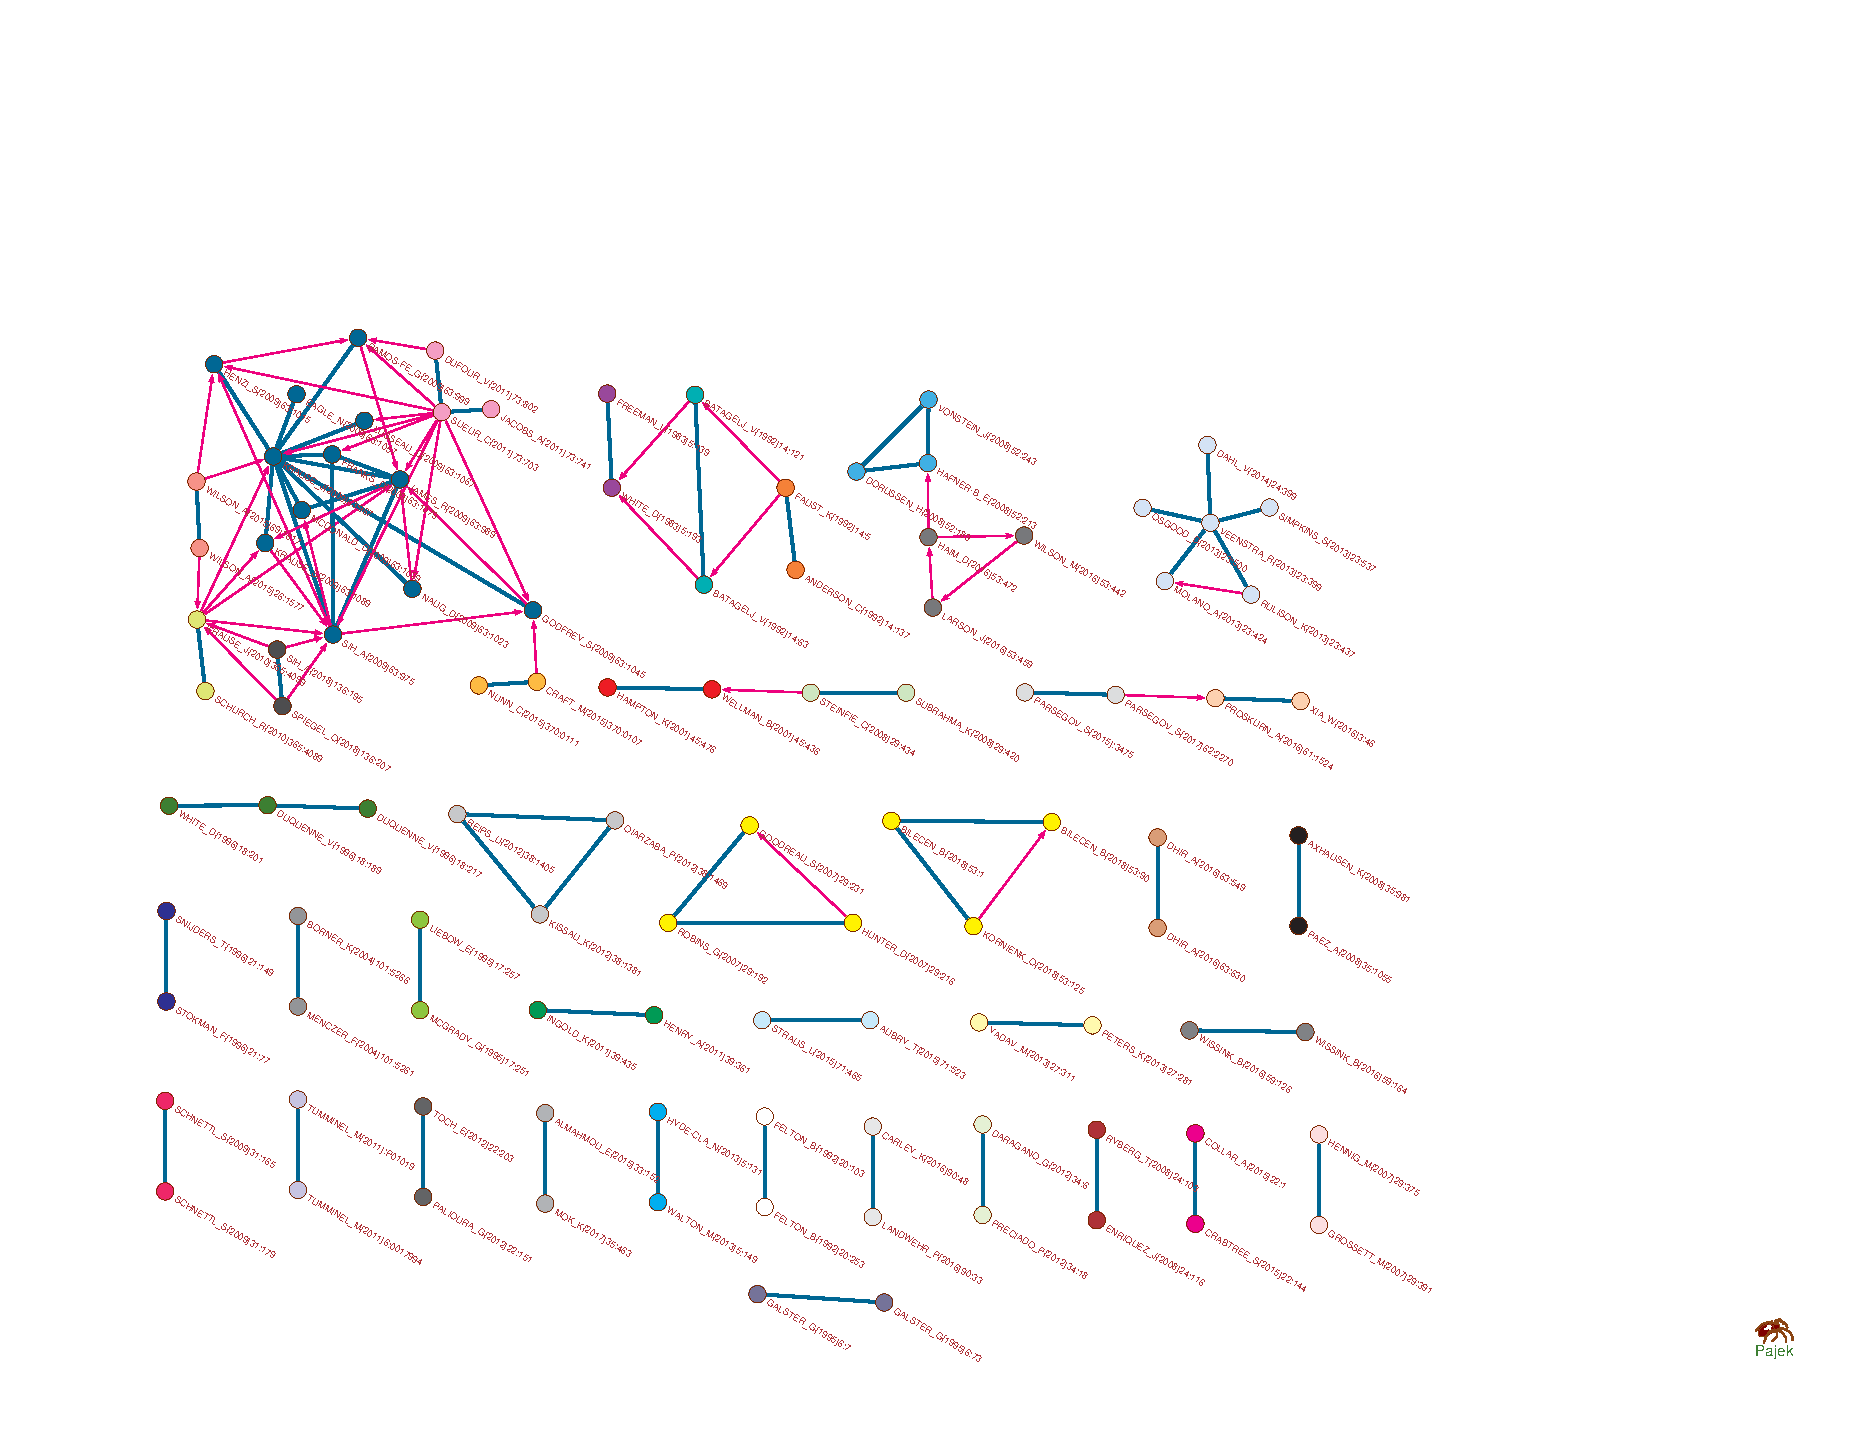
\includegraphics[width=90mm,viewport=107 179 518 434,clip=]{strong.pdf}
\end{center}

\end{frame}

\begin{frame}[fragile]
\frametitle{Preprint transformation}


 $$ \includegraphics[width=70mm,viewport=0 0 376 196,clip]{preprint.pdf} $$

\small
To transform the network  into an acyclic
network using the \href{}{preprint} transformation we applied the \Pajek's command

{\renewcommand{\baselinestretch}{0.7}
\footnotesize
\begin{verbatim}
Network/Acyclic Network/Transform/Preprint Transformation
\end{verbatim}
}

\end{frame}

\begin{frame}[fragile]
\frametitle{CPM path\label{cpmpath}}
\small 
\begin{center}
\includegraphics[width=43mm,viewport=100 40 405 550,clip=]{cpmpath1.pdf}
\end{center}
\end{frame}

\begin{frame}[fragile]
\frametitle{Key-route paths\label{taiwan}}
\small 
\begin{center}
\includegraphics[width=33mm,viewport=48 45 159 284,clip=]{taiwan.pdf}
\end{center}
\end{frame}

\begin{frame}[fragile]
\frametitle{Link islands [20 200]\label{islas}}
\small
\begin{center}
\includegraphics[width=60mm]{islandsN.pdf}
\end{center}

\end{frame}

\begin{frame}[fragile]
\frametitle{Island 10\label{islX}}
\footnotesize

\begin{center}
\includegraphics[width=60mm,viewport=45 44 481 540,clip=]{island10.pdf}
\parbox[b]{40mm}{The island 10 on 200 nodes is unreadable. We reduced its size to 150 nodes. The maximal weight is 0.5785. We get essentially the CPM path put in the context.}
\end{center}

\end{frame}



\begin{frame}[fragile]
\frametitle{\normalsize List of works on CPM path(1), main paths (2) and island (3) \\ part 1}
\label{listA}
\centerline{\includegraphics[width=105mm,viewport=124 164 718 502,clip=]{main1.pdf}}
\end{frame}

\begin{frame}[fragile]
\frametitle{\normalsize List of works on CPM path(1), main paths (2) and island (3) \\ part 2}
\centerline{\includegraphics[width=105mm,viewport=128 75 650 420,clip=]{main2.pdf}}
\end{frame}

\begin{frame}[fragile]
\frametitle{\normalsize List of works on CPM path(1), main paths (2) and island (3) \\ part 3}
\centerline{\includegraphics[width=105mm,viewport=124 164 650 498,clip=]{main3.pdf}}
\end{frame}

\begin{frame}[fragile]
\frametitle{\normalsize List of works on CPM path(1), main paths (2) and island (3) \\ part 4}
\centerline{\includegraphics[width=105mm,viewport=126 68 690 427,clip=]{main4.pdf}}
\end{frame}

\begin{frame}[fragile]
\frametitle{\normalsize List of works on CPM path(1), main paths (2) and island (3) \\ part 5}
\label{listE}
\centerline{\includegraphics[width=105mm,viewport=124 194 665 462,clip=]{main5.pdf}}
\end{frame}


\begin{frame}[fragile]
\frametitle{Island 9\label{islandB}}
\footnotesize
\begin{center}
\includegraphics[width=60mm,viewport=71 39 525 550,clip=]{island9.pdf}
\parbox[b]{40mm}{The island 9 has 44 nodes. The maximal weight is 2.416 10$^{-14}$.
Papers in this island deal with eartquake modeling. One among models is a “spring-block model”. The main journals are Phys Rev (A, E, lett), Physica A and J GEOPHYS RES.}
\end{center}
\end{frame}

\begin{frame}[fragile]
\frametitle{Island 7\label{islandC}}
\footnotesize
\begin{center}
\includegraphics[width=60mm,viewport=9 2 814 697,clip=]{island7.pdf}
\parbox[b]{40mm}{
The island 7 has 74 nodes. The maximal weight is 4.9611 10$^{-18}$.
Papers from island 7 deal with landslides (some related to earthquakes). They are using “multi-block modeling of landslides”. The main journals are SOIL DYN EARTHQ ENG, ENG GEOL and LANDSLIDES.}
\end{center}

\end{frame}

\begin{frame}[fragile]
\frametitle{Island 2\label{islandD}}
\footnotesize

\begin{center}
\includegraphics[width=60mm,viewport=65 7 725 698,clip=]{island2.pdf}
\parbox[b]{40mm}{
The island 2 has 33 nodes. The maximal weight is 2.462 10$^{-19}$.
From island.csv we see that papers from this island deal with numerical methods for computation of electromagnetic field. They use block model … Most papers are published in the journal IEEE T MICROW THEORY.}
\end{center}

\end{frame}


\section{Authors}



\begin{frame}[fragile]
\frametitle{Coauthorship networks\label{islandD}}
\footnotesize

$\Ct$   is an undirected network  obtained from $\N^T * \N$, where
\[ \N = \diag( \frac{1}{\max(1, \outdeg(p))}) \WA  \]
by symmetrization. 

Authors with the largest  $P_S$-core values in $\Ct$  are listed in Slide~\ref{maxact}. The value of an author is equal to the sum of all his/her fractional contributions to works with authors inside the core.
 For better readability loops are removed.\medskip

$\Ct'$   is an undirected network without loops obtained from $\N^T * \N'$, where
\[  \N' = \diag( \frac{1}{\max(1, \outdeg(p)-1)}) \WA , \]
by symmetrization and setting the diagonal values to 0.

Authors with the largest  $P_S$-core values in $\Ct'$ are listed in Slide~\ref{maxcoll}. The value of an author is equal to the sum of all his/her fractional collaborations with authors inside the core.\medskip

In both figures the size of nodes is proportional to its  $P_S$-core value.

\end{frame}


\begin{frame}[fragile]
\frametitle{$P_S$-cores at level 4 in $\Ct$  \label{psCoreA}}
\footnotesize
\begin{center}
\includegraphics[width=90mm,viewport=69 187 735 656,clip=]{PScoresNt.pdf}
\end{center}
\end{frame}


\begin{frame}[fragile]
\frametitle{Authors with the largest $P_S$-core values in $\Ct$}
\label{maxact}
\renewcommand{\arraystretch}{0.82}
\footnotesize
\begin{center}
\begin{tabular}{r|r|l||r|r|l}
 i & value &  author			&	 i & value &  author			\\ \hline
 1 & 21.0347 &  NEWMAN\_M	&	21 &  5.6307 &  LIU\_J		\\
 2 & 15.9653 &  BORGATTI\_S	&	22 &  5.5417 &  YANG\_J		\\
 3 & 15.9653 &  EVERETT\_M	&	23 &  5.5417 &  LESKOVEC\_J	\\
 4 & 12.5000 &  BURT\_R		&	24 &  5.5417 &  ZHANG\_J	\\
 5 & 12.5000 &  DOREIAN\_P	&	25 &  5.4432 &  HANCOCK\_E	\\
 6 & 10.4722 &  PEIXOTO\_T	&	26 &  5.4432 &  ZHANG\_Z	\\
 7 & 10.1126 &  TURCOTTE\_D	&	27 &  5.2589 &  STEINLEY\_D	\\
 8 &  8.7900 &  FERLIGOJ\_A	&	28 &  5.2589 &  BRUSCO\_M	\\
 9 &  8.7900 &  BATAGELJ\_V	&	29 &  5.2500 &  DIETERIC\_J	\\
10 &  6.5115 &  WANG\_Y		&	30 &  5.2483 &  LANCICHI\_A	\\
11 &  6.4097 &  PATTISON\_P	&	31 &  5.2483 &  FORTUNAT\_S	\\
12 &  6.4097 &  BREIGER\_R	&	32 &  5.1111 &  BOYD\_J		\\
13 &  6.2083 &  MRVAR\_A	&	33 &  5.0633 &  WANG\_X		\\
14 &  6.0292 &  ZHANG\_X	&	34 &  5.0278 &  QIAN\_X		\\
15 &  6.0292 &  WANG\_J		&	35 &  5.0208 &  WASSERMA\_S	\\
16 &  5.7500 &  PIZZUTI\_C	&	36 &  5.0000 &  OKAMOTO\_H	\\
17 &  5.7014 &  STAMATOP\_C	&	37 &  5.0000 &  JESSOP\_A	\\
18 &  5.6736 &  SUN\_P		&	38 &  4.9881 &  BARABASI\_A	\\
19 &  5.6669 &  ZHANG\_S	&	39 &  4.9775 &  KRACKHAR\_D	\\
20 &  5.6307 &  WANG\_H		&	40 &  4.9112 &  ZHANG\_H	\\ \hline
\end{tabular}
\end{center}

\end{frame}

\begin{frame}[fragile]
\frametitle{Computing $\Ct'$ in Pajek  \label{Ctp}}
\renewcommand{\baselinestretch}{0.8}
\scriptsize
\begin{verbatim}
select/read WAc network
Network/Create Vector/Centrality/Degree/Output
Network/2-Mode Network/Partition into 2 Modes
Operations/Vector+Partition/Extract Subvector [1] = V1
Vector/Create Constant Vector [5695,1] = V2
select V1 as Second vector
Vectors/Max(First,Second)
Vector/Transform/Invert
Operations/Network+Vector/Vector#Network/Output = N
select V1 as First vector
select V2 as Second vector
Vectors/Subtract (First-Second)
Vectors/Max(First,Second)
Vector/Transform/Invert
select/read WAc network
Operations/Network+Vector/Vector#Network/Output = N'
select network N
Network/2-Mode/Transpose 2-Mode
select N' as Second network
Networks/Multiply Networks [Yes]
Network/Create New Network/Transform/Remove/Loops
Network/Create New Network/Transform/Arcs -> Edges/Biderected Only/Sum
File/Network/Change Label [Ct'(WAc)]
\end{verbatim}

\end{frame}

\begin{frame}[fragile]
\frametitle{$P_S$-cores at level 3.5 in $\Ct'$  \label{psCore}}
\footnotesize
\begin{center}
\includegraphics[width=90mm,viewport=74 138 753 660,clip=]{PScoresNtt.pdf}
\end{center}

\end{frame}


\begin{frame}[fragile]
\frametitle{Authors with the  largest  $P_S$-core values in $\Ct'$}
\label{maxcoll}
\renewcommand{\arraystretch}{0.82}
\footnotesize
\begin{center}
\begin{tabular}{r|r|l||r|r|l}
    i &   value &  author          &     i &   value &  author			\\ \hline
    1 & 15.8333 &  BORGATTI\_S  &    16 &  5.0000 &  AMELIO\_A		\\
    2 & 15.8333 &  EVERETT\_M   &    17 &  5.0000 &  BAJEC\_M		\\
    3 &  7.6667 &  FERLIGOJ\_A  &    18 &  5.0000 &  SUBELJ\_L		\\
    4 &  7.6667 &  BATAGELJ\_V  &    19 &  5.0000 &  CHEN\_P		\\
    5 &  7.6667 &  MRVAR\_A     &    20 &  5.0000 &  PIZZUTI\_C	\\
    6 &  7.6667 &  DOREIAN\_P   &    21 &  5.0000 &  REICHARD\_J	\\
    7 &  6.4333 &  STEINLEY\_D  &    22 &  5.0000 &  BORNHOLD\_S	\\
    8 &  6.4333 &  BRUSCO\_M    &    23 &  4.8333 &  SALES-PA\_M	\\
    9 &  6.3333 &  YANG\_J      &    24 &  4.8333 &  GUIMERA\_R	\\
   10 &  6.3333 &  LESKOVEC\_J  &    25 &  4.5833 &  NUSSINOV\_Z	\\
   11 &  6.0000 &  LANCICHI\_A  &    26 &  4.5833 &  RONHOVDE\_P	\\
   12 &  6.0000 &  FORTUNAT\_S  &    27 &  4.3333 &  ROSVALL\_M	\\
   13 &  5.3333 &  QIAN\_X      &    28 &  4.3333 &  BERGSTRO\_C	\\
   14 &  5.3333 &  WANG\_Y      &    29 &  4.3333 &  WILSON\_R		\\
   15 &  5.0000 &  HERO\_A      &    30 &  4.3333 &  HANCOCK\_E	\\ \hline
\end{tabular}
\end{center}

\end{frame}


\begin{frame}[fragile]
\frametitle{Citations among authors}
\small
The network $\mathbf{Acite} = \WA^T * \mathbf{CiteC} * \WA$ describes the citations among authors. \medskip

The value of element  $\mathbf{Acite}[u,v]$ is equal to the number of works coauthored by $u$ that are citing a work coauthored by $v$. 

\end{frame}


\begin{frame}[fragile]
\frametitle{Citations among authors -- link islands [10 50]}
\small
\begin{center}
\includegraphics[width=90mm,viewport=64 38 830 660,clip=]{ACAislands.pdf}
\end{center}

\end{frame}

\begin{frame}[fragile]
\frametitle{Citations among authors -- link islands 17 and 16}
\small
\begin{center}
\includegraphics[width=70mm,viewport=200 120 730 820,clip=,angle=-90]{ACA16-17.pdf}
\end{center}

\end{frame}

\end{document}

%******************************************************************************
%******************************************************************************


\subsection{Collaboration}









\section{Viri}

%******************************************************************************
\begin{frame}[allowframebreaks]
\frametitle{Viri}
\footnotesize

\begin{enumerate}

  \item  \href{https://github.com/BetaNYC/Bike-Share-Data-Best-Practices/wiki/Bike-Share-Data-Systems}{List of Bike Share data portals / GitHub}
  \item  Bay Area Bike Share: \href{https://www.kaggle.com/benhamner/sf-bay-area-bike-share}{San Francisco Bay Area - Kaggle challenge}, \href{http://www.bayareabikeshare.com/open-data}{Open data}, \href{https://www.kaggle.com/c/bike-sharing-demand}{challenge}
  \item  Hubway: \href{http://hubwaydatachallenge.org/}{Boston - data challenge}
  \item  \href{https://www.citibikenyc.com/system-data}{New York}, \href{http://toddwschneider.com/posts/a-tale-of-twenty-two-million-citi-bikes-analyzing-the-nyc-bike-share-system/}{Analysis / GitHub}, \href{https://github.com/toddwschneider/nyc-citibike-data}{Data}; \href{https://www.ocf.berkeley.edu/~adityakh/2015/11/16/bike-stations-in-new-york/}{Stations}, \href{https://www.ocf.berkeley.edu/~adityakh/2015/12/14/analysis-of-the-new-york-city-bike-share-system/}{Analysis}; \href{https://www.fastcoexist.com/1682698/how-were-visualizing-new-yorks-new-bike-sharing-system}{Vis}
  \item  Divvy: \href{https://www.divvybikes.com/data}{Chicago}, \href{https://www.divvybikes.com/resources}{Info}
  \item  Indego: \href{https://www.rideindego.com/about/data/}{Philadelphia}
  \item  Capital: \href{https://www.capitalbikeshare.com/trip-history-data}{Washington, D.C.}
  \item  Healthy Ride: \href{https://healthyridepgh.com/data/}{Pittsburgh}
  \item  Budapest: \href{https://dms.sztaki.hu/bubi/}{Challenge}
  \item  \href{https://uclab.fh-potsdam.de/cf/}{London, Berlin}, \href{https://tfl.gov.uk/info-for/open-data-users/}{London}, \href{https://www.callabike-interaktiv.de/}{Berlin}
  \item  \href{http://blog.revolutionanalytics.com/2013/07/bike-sharing-in-100-cities.html}{Bike sharing in 100 cities},\href{http://ramnathv.github.io/bikeshare/}{Visualizing Bike Sharing Networks}, \href{https://github.com/ramnathv/bikeshare}{GitHub}
  \item  \href{http://nabsa.net/}{North American Bikeshare Association (NABSA)}, \href{http://nabsa.net/international-bike-share-database/}{Database}, \href{https://github.com/NABSA/gbfs}{gbfs - open standard}
  \item  \href{https://data.gov.uk/dataset/cycle-routes}{Description of the cycle path network, UK}

  \item  \href{https://bikedataproject.org/}{Bike data project}
  \item  \href{http://toddwschneider.com/posts/analyzing-1-1-billion-nyc-taxi-and-uber-trips-with-a-vengeance/}{Taxi and Uber}

  \item  Shin Chin: \href{http://blog.nycdatascience.com/student-works/detecting-anomolous-events-in-washington-dc-bike-sharing-dataset/}{Detecting Anomolous Events in Washington DC Bike Sharing Dataset}, 2016
  \item  \href{http://urbanspatialanalysis.com/origins-destinations-visualizing-bike-share-trips/}{Urban spatial analysis}, \href{http://urbanspatialanalysis.com/portfolio/project-one/}{Predict}
  \item  \href{http://www.comeetie.fr/projects.php?}{ Etienne Côme: Projects}

  \item  \href{http://velo-citta.eu/news/}{Velo-citta / news}
  \item  L Zhang, S Tang, Z Yang, J Hu, Y Shu. Demo: Data Analysis and Visualization in Bike-Sharing Systems. 2016
  \item  Vogel, Patrick: \href{http://www.springer.com/gp/book/9783319277349}{Service Network Design of Bike Sharing Systems}, 2016
  \item  \href{http://oobrien.com/bikesharemap/}{Maps}; \href{http://www.scribblelive.com/blog/2013/08/28/visualizing-bike-share-programs/}{Vis1}
  \item  \href{http://mescal.imag.fr/membres/nicolas.gast/news/2014/10/10/intership-BSS/index.html}{Internship}; \href{http://humnetlab.mit.edu/wordpress/teaching/}{Transportation systems}; \href{http://vlsstats.ifsttar.fr/}{Analysis}

  \item Patrick Vogel, Torsten Greiser, Dirk Christian Mattfeld:
Understanding Bike-Sharing Systems using Data Mining: Exploring Activity Patterns.
Procedia Social and Behavioral Sciences 20 (2011) 514–523

  \item Andreas Kaltenbrunner, Rodrigo Meza, Jens Grivolla, Joan Codina, Rafael Banchs:
Urban cycles and mobility patterns: Exploring and predicting trends in a
bicycle-based public transport system.
Pervasive and Mobile Computing 6 (2010) 455-466

  \item Jenn-Rong Lin, Ta-Hui Yang:
Strategic design of public bicycle sharing systems with service
level constraints.
Transportation Research Part E 47 (2011) 284–294

  \item Charles Bouveyron, Etienne Côme and Julien Jacques:
The discriminative functional mixture model for
a comparative analysis of bike sharing systems.
The Annals of Applied Statistics 2015, Vol. 9, No. 4, 1726–1760

  \item Oliveira, Guilherme N.; Sotomayor, Jose L.; Torchelsen, Rafael P.; et al.:
Visual analysis of bike-sharing systems.
Computers \& Graphics-UK, 60 (2016), 119-129   

  \item Matrai, Tamas; Toth, Janos:
Comparative assessment of public bike sharing systems. 
Eds.: Rafalski, L; Zofka, A:
Conference: 6th Transport Research Arena (TRA) Location: Warsaw, Poland,  Apr 18-21, 2016. 
Book Series: Transportation Research Procedia, 14 (2016), 2344-2351 

  \item Frade, Ines; Ribeiro, Anabela:
Bike-sharing stations: A maximal covering location approach.
Transportation research part a-policy and practice,  82 (2015), 216-227

  \item Zhou, Xiaolu:
Understanding Spatiotemporal Patterns of Biking Behavior by Analyzing Massive Bike Sharing Data in Chicago.
PLOS ONE  10(2015)10, e0137922 

  \item Ciancia, Vincenzo; Latella, Diego; Massink, Mieke; et al.:
Exploring Spatio-temporal Properties of Bike-sharing Systems.
Conference: 9th IEEE International Conference on Self-Adaptive and Self-Organizing Systems (SASO),
Massachusetts Inst Technol, Cambridge, MA, Sep 21-25, 2015. p. 74-79  

  \item Dell'Amico, Mauro; Hadjicostantinou, Eleni; Iori, Manuel; et al.:
The bike sharing rebalancing problem: Mathematical formulations and benchmark instances.
Omega-International journal of management science, 45 (2014), 7-19  


\end{enumerate}

WoS vrne 100 zadetkov na \texttt{"bike sharing system*"}.

\end{frame}

\section{Podatki}

%******************************************************************************
\begin{frame}[fragile]
\frametitle{Prosto dostopni podatki\\ \normalsize na mojem disku}
\small

\begin{tabular}{l|l|l|r}
Bike sharing & City             & data available  & \# of trips\\
\hline
\href{https://www.capitalbikeshare.com/trip-history-data}{Capital}      &
 Washington, D.C. & 2010/10-2016/09  & 14691090 \\
\href{https://s3.amazonaws.com/hubway-data/index.html}{Hubway}       &
 Boston           & 2011/07-2016/06 & 3930659 \\ 
\href{https://www.divvybikes.com/system-data}{Divvy}        &
 Chicago          & 2013/01-2016/06 & 7867601 \\
\href{https://www.citibikenyc.com/system-data}{Citi Bike}    &
 New York         & 2013/07-2016/09 & 33319019  \\
\href{http://www.bayareabikeshare.com/open-data}{BABS}         &
 San Francisco    & 2013/08-2016/08 & 983648 \\ 
\href{https://healthyridepgh.com/data/}{Healthy Ride} & 
Pittsburgh       & 2015/07-2016/09 & 118422  \\
\href{https://www.rideindego.com/about/data/}{Indego}       &
 Philadelphia     & 2015/04-2016/09 & 673703 \\
 \href{https://www.niceridemn.org/data/}{NiceRide} &
  Minnesota & 2010/06-2015/12  &  1808452 \\
 \href{http://cycling.data.tfl.gov.uk/}{Santander C.} &
 London &  2015/01-2016/11  &  19212558  \\
\hline
\href{https://github.com/fivethirtyeight/uber-tlc-foil-response/tree/master/uber-trip-data}{Uber} &
 New York   &  2014/04-2014/09  & \\
   &  & 2015/01-2015/06  & \\
Green & New York & 2013/08.2016/06 & 45299607 \\
Yellow & New York & 2009/01-2016/06 & 1249159178 \\
fhv & New York & 2015/01-2016/06 & 123357588 \\
\hline
\end{tabular}

\end{frame}

%******************************************************************************
\begin{frame}[fragile]
\frametitle{Podatki o postajah}
\small
North American Bike Share Association’s open data standard -- gbfs
\href{https://github.com/NABSA/gbfs}{General Bikeshare Feed Specification};
\href{https://github.com/NABSA/gbfs/blob/master/systems.csv}{uporabniki}\medskip

The Stations file is a snapshot of station locations and capacities during the reporting quarter
\begin{itemize}
 \item   Station ID
 \item     Station name
 \item     Lat/Long coordinates
 \item     Number of individual docking points at each station
\end{itemize}
V nekaterih primerih je znana tudi nadmorska višina.

Večina sistemov omogoča dobiti datoteko JSON s tekočim stanjem postaj.

\href{https://feeds.divvybikes.com/stations/stations.json}{Divvy},
\href{http://www.rideindego.com/stations/json/}{Indego}, CitiBike stations:
\href{https://gbfs.citibikenyc.com/gbfs/en/station_information.json}{info},
\href{https://gbfs.citibikenyc.com/gbfs/en/station_status.json}{status}

\end{frame}

%******************************************************************************
\begin{frame}[fragile]
\frametitle{Pobiranje stanja postaj v R-ju}
\scriptsize

\begin{verbatim}
wdir <- "C:/Users/batagelj/data/bikes/philly"
setwd(wdir)
stat <- "https://gbfs.bcycle.com/bcycle_indego/station_status.json"
num <- 0
setInternet2(use = TRUE)
p1 <- proc.time()
while (num < 5){
   num <- num+1
   fsave <- paste('status_',as.character(num),'.json',sep='')
   test <- tryCatch(download.file(stat,fsave,method="auto"),
                    error=function(e) e)
   Sys.sleep(60)
   p2 <- proc.time()
   cat(p2 - p1,'\n'); flush.console()
   p1 <- p2
}
\end{verbatim}

\end{frame}

%******************************************************************************
\begin{frame}[fragile]
\frametitle{Podatki o vožnjah}
\small

Each trip is anonymized and includes:
\begin{itemize}
 \item   Bike number
 \item     Trip start day and time
 \item     Trip end day and time
 \item     Trip start station
 \item     Trip end station
 \item     Rider type %  – Annual or Casual (24-hour or 3-day member)  If an annual member trip, it will also include the member’s home zip code
\end{itemize}
Ponekod dodatni podatki:  Gender, Year of birth

\end{frame}



%******************************************************************************
\begin{frame}[fragile]
\frametitle{Drugi viri}
\small

\textbf{Vreme}

Za ameriška mesta dobimo vremenske podatke na \href{https://www.ncdc.noaa.gov/qclcd/QCLCD}{NOAA},
\href{https://www.ncdc.noaa.gov/data-access/land-based-station-data/land-based-datasets/quality-controlled-local-climatological-data-qclcd}{Quality Controlled Local Climatological Data}

Padavine, veter, temperatura, vlažnost, tlak.\bigskip

\textbf{Zemljevidi}

Datoteke shape za posamezne kraje poiščemo na Googlu kraj shapefile

\href{https://data.cityofboston.gov/City-Services/Boston-Neighborhood-Shapefiles/af56-j7tb/data}{Boston},
\href{https://data.sfgov.org/Government/Bay-Area-Cities-Zipped-Shapefile-Format-/nghj-u9xk/data}{Bay Area Cities},
\href{http://www1.nyc.gov/site/planning/data-maps/open-data/districts-download-metadata.page}{New York},
\href{http://pittsburghpa.gov/dcp/gis/}{Pittsburgh}

%\textbf{Vreme}


    
    

\end{frame}

\section{Analize}

%******************************************************************************
\begin{frame}[allowframebreaks]
\frametitle{Analize}
\small

\begin{enumerate}

\item \href{http://hubwaydatachallenge.org/}{Hubway Data Visualization Challenge}

\item
\href{http://www.bayareabikeshare.com/datachallenge-2014}{Bay Area Bike Share Open Data Challenge 2014}

\item
Todd W. Schneider:
\href{http://toddwschneider.com/posts/a-tale-of-twenty-two-million-citi-bikes-analyzing-the-nyc-bike-share-system/}{A Tale of Twenty-Two Million Citi Bike Rides: Analyzing the NYC Bike Share System}.\medskip

\item
Aditya Khandekar:
\href{https://www.ocf.berkeley.edu/~adityakh/2015/12/14/analysis-of-the-new-york-city-bike-share-system/}{Analysis of the New York City bike share system}, December 2015

\item
Jackson Whitmore: \href{http://suds-cmu.org/2016/04/21/whats-happening-with-healthy-ride/}{What’s happening with Healthy Ride?}, April 2016.

\item  George Lejnine: \href{http://lejnine.com/bike_analysis.html}{A Study of HealthyRide Pittsburgh Data}, April 2016.

\item   Lauren Renaud: \href{http://www.laurenrenaud.com/blog/2016/2/1/healthy-ride-pgh-bike-share-data}{Tableau: Healthy Ride PGH Bike Share Data}, February 2016.

\item  Southwestern Pennsylvania Commission: \href{http://www.spcregion.org/trans_multi_atp.shtml}{Healthy Ride Pittsburgh Bike Share Maps}, September 2015.

\item Sydney Brownstone:
\href{https://www.fastcoexist.com/1682698/how-were-visualizing-new-yorks-new-bike-sharing-system}{How we're visualizing New York's new bike sharing system}, November 2014.

\item Todd W. Schneider:
\href{http://toddwschneider.com/posts/analyzing-1-1-billion-nyc-taxi-and-uber-trips-with-a-vengeance/}{Analyzing 1.1 Billion NYC Taxi and Uber Trips, with a Vengeance},


\end{enumerate}

\end{frame}

%******************************************************************************
\begin{frame}[fragile]
\frametitle{Prikazi}
\normalsize
Statični: omrežje, matrika

\href{http://hubwaydatachallenge.org/submission/9/}{Graf 1}; 
\href{http://hubwaydatachallenge.org/submission/52/}{Graf 2};
\href{http://hubwaydatachallenge.org/submission/1/}{Flow};
\href{http://hubwaydatachallenge.org/submission/39/}{Matrika}

 \href{http://lejnine.com/bike_analysis.html}{Med postajami - krožno}
 \bigskip
 
 
Dinamični: \href{https://www.youtube.com/watch?v=JMBXdKj4iDQ}{zemljevid}, 
\href{http://russellgoldenberg.com/hubway/}{abstraktni}


\end{frame}


%******************************************************************************
\begin{frame}[fragile]
\frametitle{Statistične analize}
\small
Predvsem razne porazdelitve voženj glede na različne dejavnike.

\href{http://suds-cmu.org/2016/04/21/whats-happening-with-healthy-ride/}{Pitts};
\href{http://thfield.github.io/babs/}{Bay};
\href{http://hubwaydatachallenge.org/submission/22/}{Boston};
\href{http://toddwschneider.com/posts/a-tale-of-twenty-two-million-citi-bikes-analyzing-the-nyc-bike-share-system/}{NYC BSS;};  \href{http://toddwschneider.com/posts/analyzing-1-1-billion-nyc-taxi-and-uber-trips-with-a-vengeance/}{NYC Taxi and Uber}\medskip

Vreme: temperatura: dan - noč, poletje- zima; padavine. Taxi = dežnik? \medskip


Letno obnašanje (temperatura), tedensko obnašanje (dan, delavnik/weekend), dnevno obnašanje (ura, zjutraj / dopoldne /
opoldne / popoldne / zvečer / ponoči). \href{http://ariofsevit.com/hubway/}{tedensko};  \href{http://lejnine.com/bike_analysis.html}{vožnje po dnevih}\medskip


Člani/nečlani, trajanje vožnje, spol, starost uporabnika, postajo, hitrost. Vpliv terena (višine).
\href{http://hubwaydatachallenge.org/submission/10/}{starost}\medskip


Sistemske prestavitve koles je mogoče razpoznati po tem, da se naslednja vožnja začne drugje kot se
je končala zadnja.

\href{http://hubwaydatachallenge.org/submission/55/}{Prihodi/odhodi};
\href{http://zsobhani.github.io/hubway-team-viz/}{Boston};
\href{http://hubwaydatachallenge.org/submission/35/}{Spreminjanje uravnoteženosti} \medskip

Zahtevnejše: \href{https://www.kaggle.com/jlinsche/d/benhamner/sf-bay-area-bike-share/count-prediction/discussion}{SF Bay Area: count prediction}

\end{frame}


\section{Kolesarska omrežja}

%******************************************************************************
\begin{frame}[fragile]
\frametitle{Operacijske raziskave}
\small


 problem nameščanja postaj:
 
 \begin{itemize}
   \item Frade, Ines; Ribeiro, Anabela:
Bike-sharing stations: A maximal covering location approach.
Transportation research part a-policy and practice,  82 (2015), 216-227
 \end{itemize}

 
 problem uravnotežanja dostopnosti koles:
  \begin{itemize}
  \item Dell'Amico, Mauro; Hadjicostantinou, Eleni; Iori, Manuel; et al.:
The bike sharing rebalancing problem: Mathematical formulations and benchmark instances.
Omega-International journal of management science, 45 (2014), 7-19 
 \end{itemize}

\end{frame}

\begin{frame}[fragile]
\frametitle{Kolesarska omrežja}
\small
Podatke o izmenjavi koles lahko obravnavamo kot časovno omrežje:

Vozlišča - postaje: ime, lokacija, zmogljivost, (stanje)

Povezave - vožnje: od, do, začetek, konec, kolo (relacija), članstvo, spol \medskip

Iz njega lahko pridobimo veliko izpeljanih omrežij. Glede na količino podatkov utegne biti časovno
potratno.\medskip

Problem: podatki o vozliščih so statitični ali občasni (delna neusklajenost z vožnjami). Mogoče bi
jih bilo zbirati sproti s spleta. \medskip

Granulacija: 5 min, 15 min, ura, del dneva, dan, teden, mesec, četrtletje, leto \medskip

Porazdelitve (z omejitvami)\\
v vozliščih: uravnoteženost \\
in na povezavah: začetek vožnje, trajanje vožnje

\end{frame}

\begin{frame}[fragile]
\frametitle{Kolesarska simbolna omrežja}
\small
Simbolno omrežje dobimo tako, da vozliščem in povezavam priredimo simbolne vrednosti -- porazdelitve.
Možnih je več porazdelitev na povezavah, npr.: \medskip\\
odhodov: (časovni interval, število voženj z začetkom v njem),\\
toka: (časovni interval, število voženj dejavnih v njem,)\\
trajanj: (časovni interval, število voženj s trajanjem v njem), itd.\medskip\\
in v vozliščih, npr.:\medskip\\
odhodov: vsota porazdelitev odhodov po povezavah,\\
odtoka/pritoka: vsota porazdelitev tokov na povezavah,\\
``deficita'' (uravnoteženost), itd.\medskip

Te porazdelitve lahko s programom \href{https://rdrr.io/rforge/clamix/}{Clamix} razvrstimo v skupine in tako dobimo voditelje -- tipična obnašanja 
v omrežju. Zanimivi so tudi elementi (vozlišča/povezave), ki najbolj odstopajo od svojih voditeljev ali pa so
neuvrščeni. 


\end{frame}

\end{document}

%******************************************************************************
%******************************************************************************

%******************************************************************************

\begin{frame}[plain]
\end{frame}

\begin{frame}[plain]
\end{frame}




